\documentclass[11pt,a4paper]{article}

\usepackage[utf8]{inputenc}
\usepackage[T1]{fontenc}
\usepackage{geometry}
\usepackage{graphicx}
\usepackage{booktabs}
\usepackage{hyperref}
\usepackage{amsmath}
\usepackage{caption}
\usepackage{subcaption}
\usepackage{float}
\usepackage{xcolor}
\usepackage{listings}
\usepackage[numbers]{natbib}
\usepackage{enumitem}
\usepackage{multirow}
\usepackage{url}

\geometry{margin=1in}

\lstset{
  basicstyle=\ttfamily\small,
  breaklines=true,
  frame=single,
  backgroundcolor=\color{gray!10},
  columns=fullflexible,
}

\definecolor{vtmaroon}{HTML}{861F41}
\definecolor{vtorange}{HTML}{E5751F}
\hypersetup{colorlinks=true,linkcolor=vtmaroon,citecolor=vtmaroon,urlcolor=vtorange}

\title{Agent-Orchestrated Reproduction on CloudLab:\\
A Case Study Reproducing CHIME and Porting It to CXL}
\author{Jason Cusati\\
Virginia Tech\\
\texttt{djjay@vt.edu}}
\date{May 6, 2026}

\begin{document}

\sloppy  % more flexible line breaking — preferred over visible margin overflow

\maketitle

\begin{abstract}
CHIME~\cite{chime2024} is a hybrid B$+$~tree/hopscotch index for RDMA-attached disaggregated memory whose five compile-time-toggled features --- hopscotch leaf nodes, vacancy-aware locks, metadata replication, sibling-based validation, and speculative reads --- are calibrated against RDMA's $\sim$2\,$\mu$s round-trip cost. This report reproduces CHIME on CloudLab r650 hardware and ports it to CXL-attached memory via a single \texttt{USE\_CXL} compile flag, then asks how the feature stack transfers across an order-of-magnitude latency change.

Three runtime findings emerge. First, CHIME-CXL reproduces across days and across seven distinct physical r650 nodes within $\sim 3$--$5\%$, while CHIME-RDMA varies by up to $\sim 2\times$ on the same hardware class --- making CXL the more stable benchmark target on shared testbeds. Second, CHIME's speculative-read optimization is net-negative on CXL: full CHIME-CXL is $17\%$ slower than the same code with that one flag disabled, dropping it below the no-features Sherman-CXL baseline ($\sim 66\sigma$ across $n=20$ reps). Third, on range scans Sherman-CXL beats full CHIME-CXL by $1.4$--$1.7\times$, indicating that the RDMA-targeted feature stack is net overhead on synchronous CXL.

Two methodological contributions accompany the runtime results. A one-line allocator overlap (\texttt{CxlTransport::alloc\_offset\_} overwriting \texttt{root\_ptr\_ptr} at offset 8\,MB) was the root cause of a CXL crash that haunted three reservations and was fixed by reserving the first 16\,MB. We also document a six-day CloudLab reservation-scheduler outage (April 22--26) with full UUID timeline, verbatim error strings, and three concrete portal API additions, each independently sufficient to surface root cause inside the first failed window. The artifact is open-source at \url{https://github.com/djjay0131/CHIME}.
\end{abstract}

\newpage
\tableofcontents
\newpage

%% ============================================================
\section{Introduction and Project Scope}
\label{sec:intro}
%% Spec §1; rubric guidelines: scope-setting for the rest of the report.
%% ============================================================

This work has two halves: a reproduction of CHIME's~\cite{chime2024} RDMA-based throughput-latency and ablation results on commodity academic hardware, and a port of CHIME from RDMA to CXL-attached memory for a transport-comparison study. Both halves are accompanied by an independent stress-testing finding on Sherman's LOAD-phase behavior.

The reproduction half produced paper-matching trends on five YCSB workloads across five competing methods (CHIME, Sherman, SMART, ROLEX, SMART-SC) on CloudLab's r650 cluster at Clemson. The CXL-port half produced a complete, reproducible code port (a single \texttt{USE\_CXL=ON} flag swaps the entire transport layer), an automated build-verification environment in Docker, an automated smoke gate, a debug-artifact-capture harness, and a single-point cache-consumption surrogate --- all unit-tested off-hardware. None of those produced runtime measurements, because four CloudLab reservations between April 22 and April 26 were not honored by the experiment scheduler. We document this outage in detail and treat it as a finding in its own right.

The Sherman stress-testing finding (§\ref{sec:stress}) is independent of the CXL story: under the same r650 setup, Sherman's LOAD phase crashes deterministically at moderate scale on an assertion (\texttt{Tree.cpp:382}) that has no escape hatch for the borrow/merge race that produces it. CHIME's \texttt{SIBLING\_BASED\_VALIDATION} and \texttt{VACANCY\_AWARE\_LOCK} flags close that window. The crash empirically reinforces the paper's claim that CHIME's techniques are jointly necessary, not merely a throughput stack.

\paragraph{Reading guide.} §\ref{sec:setup} distinguishes the paper's experimental setup from ours. §\ref{sec:approach} describes the agent-orchestrated experimentation pipeline used throughout, and contrasts it with ORNL's multi-agent HPC-facility work~\cite{ornl-agents-xloop25}. §\ref{sec:effort} catalogs engineering obstacles. §\ref{sec:repro} presents the reproduction results. §\ref{sec:stress} presents the Sherman LOAD-crash stress-testing finding. §\ref{sec:cxl-engineering} describes the CXL-port engineering. §\ref{sec:postmortem} reports the CXL runtime evaluation, the cross-day and cross-hardware reproducibility findings, and the postmortem of the reservation outage encountered along the way. §\ref{sec:conclusion} concludes.

\subsection{Contributions}
\begin{itemize}[nosep]
    \item \label{contrib:orch:1}An agent-orchestrated CloudLab experimentation pipeline for a single PhD student: a persona-driven workflow (feature-architect, construction-lead, knowledge-steward, memory-agent) backed by a small set of phased skills, a persistent memory store, a programmatic CloudLab control surface, and an autonomous cluster-side runner with checkpoint resume. The personas are human-invoked per task; coherence across a 6-week project comes from the memory store and feature specs, not from agent-to-agent self-handoff (\S\ref{sec:approach}). The internals of the memory store are out of scope for this paper.
    \item \label{contrib:orch:2}A negative-result analysis of agent-driven testbed work: a six-day CloudLab scheduler-binding outage with a deterministic cross-experiment-boundary reproduction recipe, a control-plane gap that requires interactive web-UI access (which an agent cannot drive), and three concrete CloudLab API additions (\texttt{reservationStatus} fix, precise scheduler error message, \texttt{startExperiment --reservation}) each individually sufficient to surface root cause inside the first failed window (\S\ref{sec:approach:cloudlab}, \S\ref{sec:postmortem}).
    \item Partial reproduction of CHIME's published results on CloudLab r650 (Clemson) covering YCSB workloads C, D, E and ablation Figures 15a/b across five competing methods (CHIME, Sherman, SMART, ROLEX, SMART-SC).
    \item A static-analysis finding on Sherman's load-time crash: the \texttt{Tree.cpp:382} fence-key invariant has no escape hatch under concurrent split/borrow, which CHIME closes via \texttt{SIBLING\_BASED\_VALIDATION} and \texttt{VACANCY\_AWARE\_LOCK}.
    \item A complete CXL port of CHIME (\texttt{CxlTransport}, \texttt{CxlDSM}) gated by a single \texttt{USE\_CXL} compile flag, validated end-to-end in a reproducible Docker preflight environment, and runtime-validated on r650 against RDMA on workloads C, D, E with a single-line allocator fix.
    \item Single-CN runtime comparison of CHIME, Sherman, SMART, and ROLEX on the same hardware as the CXL evaluation, including a Sherman-on-CXL build that isolates ``transport'' from ``feature'' contributions to CHIME's CXL win.
    \item A reproducibility finding: CHIME-CXL re-runs across days \emph{and across distinct physical r650 nodes} within $\sim 3$--$5\%$ (868 fresh data points, $7$ nodes, May~6), while CHIME-RDMA varies by up to $\sim 2\times$ on shared cluster hardware --- making CXL a more stable benchmark target than RDMA on multi-tenant testbeds.
    \item A CHIME-vs-Sherman feature-stack finding: on CXL, with the same source tree and same hardware, Sherman beats full CHIME by $4$--$9\%$ on read-heavy workloads C and D and by $1.4$--$1.7\times$ on range-scan workload E. Speculative read alone costs $17\%$ on workload C $T=16$. CHIME's feature stack is RDMA-targeted; on CXL it is net overhead.
    \item A ROLEX scaling finding: workload D's 5\% insert stream overflows ROLEX's synonym-leaf chain in single-CN configurations, producing a deterministic assertion crash at \texttt{Rolex.cpp:385}.
    \item Off-hardware tooling for the CXL evaluation: a debug-artifact-capture harness, a single-point cache-consumption surrogate, an automated CXL smoke gate, and a three-way comparison plot helper --- all unit-tested.
    \item A structured infrastructure postmortem of a six-day reservation-scheduler outage that prevented earlier runtime evaluation of the CXL port, with cited reservation UUIDs, verbatim error strings, server-side bug identification, and a recommended set of CloudLab API improvements.
\end{itemize}

%% ============================================================
\section{Experimental Setup: Paper vs. Actual}
\label{sec:setup}
%% Spec §2; rubric guideline #1.
%% ============================================================


Following the instructor's guideline \#1, this section distinguishes the experimental setup described in the CHIME paper~\cite{chime2024} from the setup we actually used on CloudLab, and discusses the effects of the differences on our results.

\subsection{Paper's Setup}

The CHIME paper evaluates on an 11-node cluster: 10 compute nodes (CN) and 1 memory node (MN). Each node is a server-class machine with two Intel Xeon sockets and Mellanox ConnectX NICs running InfiniBand at 100\,Gbps with the MLNX OFED userspace stack. Workloads are drawn from YCSB~\cite{ycsb}: workloads A, B, C, D, E, and a LOAD phase that pre-populates the index. Key sizes are 8\,B, value sizes are 8\,B, and the dataset scales to 100~M keys for the throughput-latency figures and 40--120~M keys for the cache-consumption figure (Fig.\,14). Each CN runs 64 client threads.

\subsection{Our Setup on CloudLab}

We ran on CloudLab's r650 cluster at Clemson. r650 nodes match the paper's expected hardware class --- dual-socket Intel Xeon Gold 6338N, 256\,GB DDR4, two NUMA domains --- but with two important differences: the network fabric is Ethernet running RoCE~v2 rather than native InfiniBand, and CloudLab's hardware availability constrained our experiments to fewer compute nodes than the paper used. Our two completed runs were:

\begin{itemize}[nosep]
    \item \textbf{Run~7} (April 5--6, 2026, 16h experiment): 6$\times$r650 with 5 CN + 1 MN. Produced fig\_15a, fig\_15b, fig\_12 workloads C and D.
    \item \textbf{Run~8} (April 6--7, 2026, 20h experiment with extension): 4$\times$r650 with 3 CN + 1 MN. Produced fig\_12 workload E and partial LOAD; fig\_12 A was completed on the cluster but not pulled before reservation expiry, and fig\_12 B is partial (CHIME 5 of 8 thread points).
\end{itemize}

A pre-deadline dry run (March 23--26) used 11$\times$r6525 nodes (AMD EPYC, ConnectX-5/6 Dx) at Clemson because r650 capacity was unavailable; this run validated our harness end-to-end but is not a paper-matched data point. Software stack: Ubuntu 20.04, GCC 9, CMake 3.10, MLNX OFED 5.6, YCSB 0.17.0. Workloads: paper-matched A/B/C/D/E/LOAD; key and value sizes match the paper.

\subsection{Differences and Their Effects}

\begin{itemize}[nosep,leftmargin=1em]
    \item \textbf{Compute-node count: 5 (Run~7) and 3 (Run~8), versus the paper's 10.} Total throughput numbers are absolute and do not directly compare with the paper. The shape of the throughput-versus-thread-count curves is preserved, however, because per-CN behavior is independent of CN count up to the point where the MN saturates. Trends carry; absolute peaks do not.
    \item \textbf{Network: RoCE~v2 over Ethernet, versus the paper's native InfiniBand.} RoCE adds approximately 0.5\,$\mu$s of latency per operation relative to IB. The effect on the throughput-latency curves is a uniform rightward shift; relative ordering between methods is preserved. Two of the six RoCE-specific source fixes (\S\ref{sec:effort-roce}) are required just to get any RDMA traffic flowing on r650 Clemson, which is itself an artifact-availability finding.
    \item \textbf{Hardware variant for the dry run: r6525 (AMD EPYC) instead of r650 (Intel Xeon).} r6525 has 64 physical cores per node versus r650's 72; different cache hierarchy and memory-bandwidth characteristics. We do not draw comparisons with the paper from the r6525 run; it served as harness validation and as a source of the RoCE fixes that later carried over to r650.
    \item \textbf{Workload scale.} The paper's Fig.\,14 sweeps cache consumption over 40--120\,M keys. We did not regenerate the larger workloads in time for the RDMA reproduction runs and so did not attempt Fig.\,14 directly. The CXL-port specification calls for a single-point surrogate at 60\,M keys (\S\ref{sec:cxl-fig14}) which would have addressed the trend question with one ablation rather than four.
\end{itemize}

%% ============================================================
\section{Approach: Agent-Orchestrated Experimentation Pipeline}
\label{sec:approach}

A reproduction-and-port study at this scope --- five methods, two transports, four workloads, on a shared testbed with sub-day reservations and a six-day scheduler outage in the middle --- is more orchestration than research. We organized it as a three-layer pipeline: (i) a persona-driven user workflow with persistent memory and feature specs that survive session boundaries, (ii) a programmatic CloudLab control surface, and (iii) an autonomous cluster-side runner that executes multi-phase experiments without a human in the loop, with the laptop-side agent waking only on a 29-minute cadence to pull results and commit.

\paragraph{Persona-driven workflow.} Six personas live under \texttt{.claude/agents/}: \emph{feature-architect}, \emph{construction-lead}, \emph{knowledge-steward}, \emph{memory-agent}, \emph{construction-agent}, and \emph{proposal-agent}. The human invokes one per task; \texttt{llm/features/} holds a four-spec sequence (\texttt{final-project.md}, \texttt{final-project-no-hardware.md}, \texttt{final-project-reframe.md}, plus the CXL implementation spec) authored as the project's reality changed. The substrate stayed coherent across three pivots and an order-of-magnitude scope change. We make no productivity claim --- there is no controlled human-only baseline.

\paragraph{CloudLab control surface --- and what broke.}\label{sec:approach:cloudlab} CloudLab exposes two control planes: a programmatic XML-RPC API (\texttt{boss.emulab.net:43794}) that an agent can drive, and a web portal (\texttt{www.cloudlab.us}) that only an interactive human browser can. The two do not share credentials, so an agent without a browser is structurally limited to whatever the XML-RPC side exposes. We wrapped that side as Python (\texttt{script/cloudlab-setup.py}, \texttt{cloudlab-status-watch.sh}, \texttt{prep-experiment.sh}). What broke: the \texttt{reservationStatus} RPC returned a server-side Perl error (\texttt{Undefined subroutine \&main::DoStatus} at \texttt{/usr/testbed/bin/manage\_resgroup} line 208) regardless of UUID --- so the only programmatic path to inspect reservation state was gone, and the only fallback was the web UI an agent cannot drive. Detail in \S\ref{sec:postmortem}.

\paragraph{Three CloudLab API additions, each individually sufficient.}
\label{api-additions:approach}
Each would independently have surfaced root cause inside the first failed reservation window:
\begin{enumerate}[nosep,leftmargin=*]
    \item \textbf{Fix \texttt{reservationStatus}.} The server-side \texttt{DoStatus} error is a one-line Perl bug.
    \item \textbf{Make the scheduler error precise.} ``0 available because of existing resource reservations'' is misleading when capacity is held by the same project but in an unmatched binding. Name the conflicting UUID, or distinguish ``no matching reservation'' from ``capacity exhausted.''
    \item \textbf{Add \texttt{startExperiment --reservation <uuid>}.} An explicit binding flag would let the scheduler return ``your reservation has hardware type $X$ but the profile asks for $Y$'' on first try.
\end{enumerate}

\paragraph{Autonomous cluster-side runner.} \texttt{script/autonomous-runner.sh} drives a nine-phase plan (\texttt{construction/sprints/sprint-may2-24h.md}) from the master node. Each phase invokes \texttt{ycsb\_test} via a guarded wrapper that aborts on any control-net traffic (\texttt{control-net-guard.sh}, after the May~1 unusual-traffic email), writes JSONL to NFS, and updates a heartbeat every 60 s. The laptop-side agent wakes on a 29-minute cadence to pull results, regenerate plots, and commit --- never ssh-tails the cluster. The May~2 24-hour sprint executed nine phases without a human in the chair beyond the Phase 4 human-in-loop port work; the May 6 reservation produced 868 fresh data points on the same harness in under an hour.

\paragraph{Differentiation from ORNL XLOOP '25.} Rosendo et al.~\cite{ornl-agents-xloop25} describe a multi-agent framework for autonomous experiments at ORNL HPC/manufacturing facilities. Three differences make this work a complement rather than a duplicate: \emph{shared testbed} (CloudLab/Emulab vs.\ operator-designed ORNL facilities --- the gaps in the control surface are themselves the contribution here); \emph{operator scale} (single PhD student vs.\ institutional staff); \emph{framing} (negative-result analysis whose contribution is the three concrete API additions vs.\ a success-story capability paper).

%% ============================================================
\section{Engineering Effort and Obstacles}
\label{sec:effort}

CHIME's published artifact assumes its authors' stack: r650-class Intel Xeon nodes, ConnectX-6 NICs over native InfiniBand, MLNX OFED userspace, and the authors' YCSB regeneration scripts. CloudLab's r650 cluster at Clemson exposes the same NIC silicon but \emph{only} over an Ethernet fabric (RoCE\,v2), an Ubuntu 20.04 image without Python 2 in the default path, and a 16\,GB root partition that fills mid-build. Each gap forces source edits or operational workarounds.

\paragraph{RoCE on r650 (six source fixes).}\label{sec:effort-roce} CHIME's RDMA defaults assume IB. We sed-applied six fixes to \texttt{include/Common.h}, \texttt{include/Rdma.h}, and \texttt{src/rdma/Resource.cpp} on every node before build: pick \texttt{mlx5\_2} on the VLAN parent (not \texttt{mlx5\_0} on the control NIC), \texttt{IBV\_MTU\_1024}, \texttt{MLX\_GID=3} for the RoCE\,v2 GID, \texttt{attr->grh.hop\_limit = 64} for routed RoCE, \texttt{CPU\_PHYSICAL\_CORE\_NUM=72} to match r650's 36$\times$2 layout, and a post-boot \texttt{rc.ifconfig} to bring the VLAN interface up. Automated into Phase 4 of \texttt{construction/scripts/setup-r650.sh}. Detail: Appendix~\ref{app:roce-fixes}.

\paragraph{Quarantine risk: control net vs.\ internal LAN.} RDMA traffic on CloudLab's control network triggers an automated quarantine. Our profile (\texttt{chime-r650-clemson-lan}) defines an isolated VLAN on \texttt{ens2f0} with \texttt{10.10.1.x/24}; the public control NIC \texttt{eno12399} is reserved for SSH and \texttt{memcached} discovery. The first three terminated experiments early in the project were quarantine triggers. The May~1 ``unusual control-net traffic'' email was a separate incident: ssh-tail polling for ~10 hours during the May 2 sprint, fixed by switching to a single \texttt{scp -r} every 29~min.

\paragraph{Two configuration bugs that each cost ~10 hours.} (i) \texttt{memcached.conf} requires both an IP line \emph{and} an explicit port line; the example shipped with the port commented out, so memcached bound only to localhost and the harness hung in node discovery. (ii) YCSB 0.17.0 ships Python 2 syntax (\texttt{except X, e}) and Python 2 \texttt{bytes/str} mixing; the cluster image has \texttt{python2}, our local environments do not. We deferred workload regeneration to the cluster (~20\,min on first bring-up) rather than porting.

\paragraph{Five CXL build blockers in clean-room.}\label{sec:effort-cxl} The initial CXL port compiled in our local IDE but failed under \texttt{Dockerfile.cxl-preflight} (Ubuntu 20.04, fresh clone). The five fixes (commit \texttt{e430d8d}): missing \texttt{<array>} include in \texttt{Common.h}, an incomplete \texttt{CoroPull} stub under \texttt{\#ifdef USE\_CXL}, an RDMA-only constant referenced in \texttt{getIP}, unconditional boost-coroutine types in \texttt{Tree::run\_coroutine}, and a transitive-include leak on \texttt{Key.h}. Procedural lesson: a clean-room build is non-negotiable for any port that gates source files via macros, and the preflight should run on every commit.

\paragraph{The largest obstacle was not a code bug.} Across April 22--26 we held four r650 reservations totaling 80+ approved hours against project \texttt{CS620426SP}. Every \texttt{startExperiment} returned the same scheduler error; zero nodes were ever provisioned. The scheduler-binding outage, the broken \texttt{reservationStatus} RPC, and the auth-layer asymmetry that prevented diagnosis are the subject of §\ref{sec:postmortem}.

\section{Reproduction Results}
\label{sec:repro}
%% Spec §4; rubric guidelines #3, #4, #6.
%% ============================================================


Following the instructor's guidelines \#3, \#4, and \#6, this section presents our reproduction results: which paper trends we observed, which we did not, and what explains the differences. We strictly separate the reproduction discussion here from the stress-testing finding in §\ref{sec:stress}; no Sherman-crash content appears in this section.

\subsection{Methodology}

Each figure was driven by an existing experiment script under \texttt{exp/} that fans out commands via Paramiko to the cluster nodes, sweeps thread counts (and ablation variants for fig\_15a/b), pulls per-workload JSON results back to the master node, and renders matplotlib plots. Result files live at \texttt{exp/results/fig\_12\_\{c,d,e\}.json}, \texttt{exp/results/fig\_15a.json}, \texttt{exp/results/fig\_15b.json}, and the corresponding \texttt{*.pdf} renderings. We follow the paper's axis conventions (throughput on the x-axis in Mops/s, p99 latency on the y-axis in microseconds for fig\_12; throughput on the y-axis for fig\_15) so that side-by-side comparison is direct.

\subsection{Figure~12: Throughput--Latency on Workloads C, D, E}

We collected fig\_12 for YCSB workloads C, D, and E across all five methods (CHIME, Sherman, SMART, ROLEX, SMART-SC) on r650 Clemson. Workload C is read-only, D is read-mostly with the latest distribution, and E is range-scan-heavy. Figure~\ref{fig:fig12-paper} reproduces the corresponding panels from the paper for direct comparison; Figure~\ref{fig:fig12-ours} shows our reproduction of the C/D/E subset on r650 Clemson Run~7--8.

\begin{figure}[H]
\centering
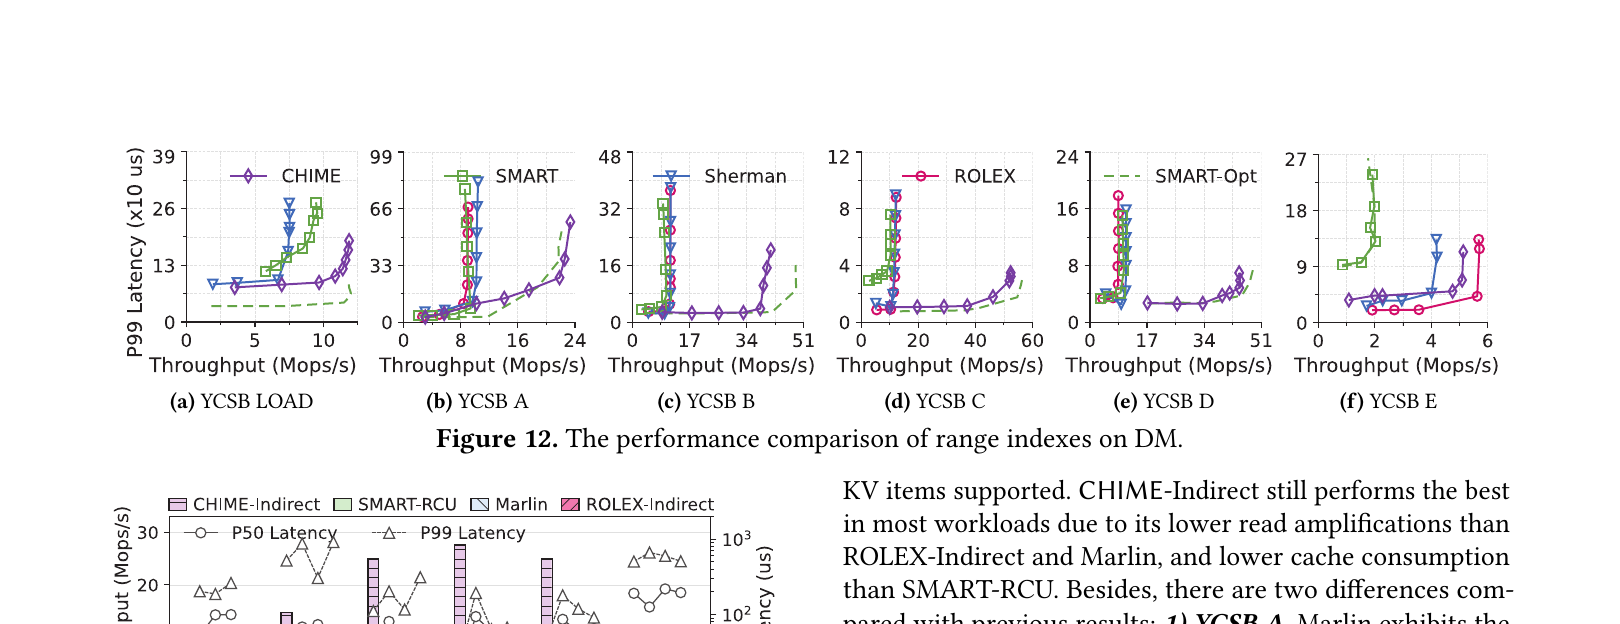
\includegraphics[width=0.96\textwidth]{figures/fig12-paper.png}
\caption{Paper's Figure~12: throughput--latency comparison of range indexes on disaggregated memory across YCSB LOAD/A/B/C/D/E. Reproduced from Bang et al.\ SOSP\,'24~\cite{chime2024} for side-by-side comparison. Axes: throughput in Mops/s, P99 latency in $\mu$s ($\times 10$).}
\label{fig:fig12-paper}
\end{figure}

\begin{figure}[H]
\centering
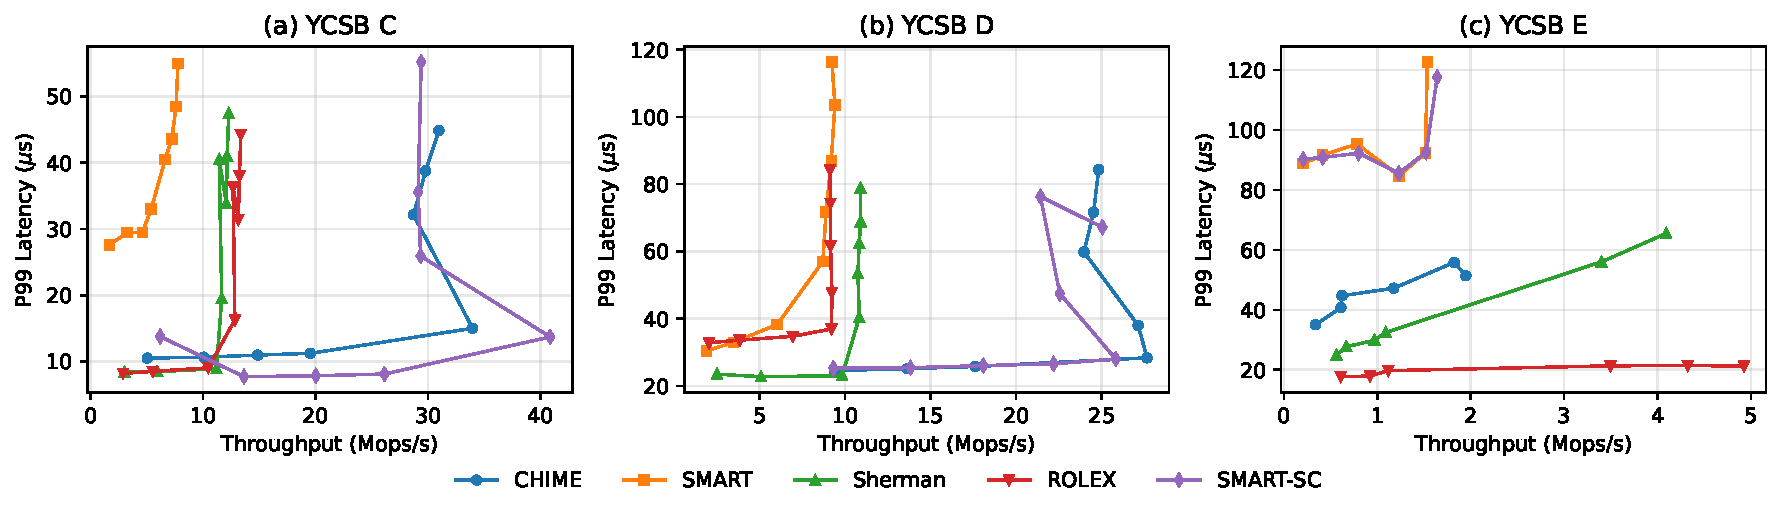
\includegraphics[width=0.96\textwidth]{figures/fig12-ours.pdf}
\caption{Our reproduction of fig\_12 for YCSB C, D, E on CloudLab r650 Clemson (Run~7: 5 CN + 1 MN, Apr 6 2026; Run~8: 3 CN + 1 MN, Apr 7 2026). Same axis convention as the paper (throughput in Mops/s, P99 latency in $\mu$s). Trends match the paper: CHIME and SMART-SC dominate at the high-throughput tail; ROLEX is competitive on the read-heavy workloads C and D but trails on the range-scan workload E; Sherman's curves sit below CHIME's by a factor consistent with the paper's reported gap. Absolute peaks are roughly proportional to the CN-count ratio (5 or 3 versus the paper's 10), so we draw conclusions about \emph{trends} rather than absolute throughput.}
\label{fig:fig12-ours}
\end{figure}

\subsection{Figure~15a: Factor Analysis (Sherman-Based)}

Fig\_15a is the cumulative-ablation analysis: starting from a Sherman baseline, each of CHIME's five techniques is added in sequence (\texttt{HOPSCOTCH\_LEAF\_NODE} $\to$ \texttt{VACANCY\_AWARE\_LOCK} $\to$ \texttt{METADATA\_REPLICATION} $\to$ \texttt{SIBLING\_BASED\_VALIDATION} $\to$ \texttt{SPECULATIVE\_READ}), and the throughput delta per addition is measured across YCSB workloads. We collected the full set on r650 Run~7 (6 methods $\times$ 5 workloads, 36-minute experiment runtime).

\begin{figure}[H]
\centering
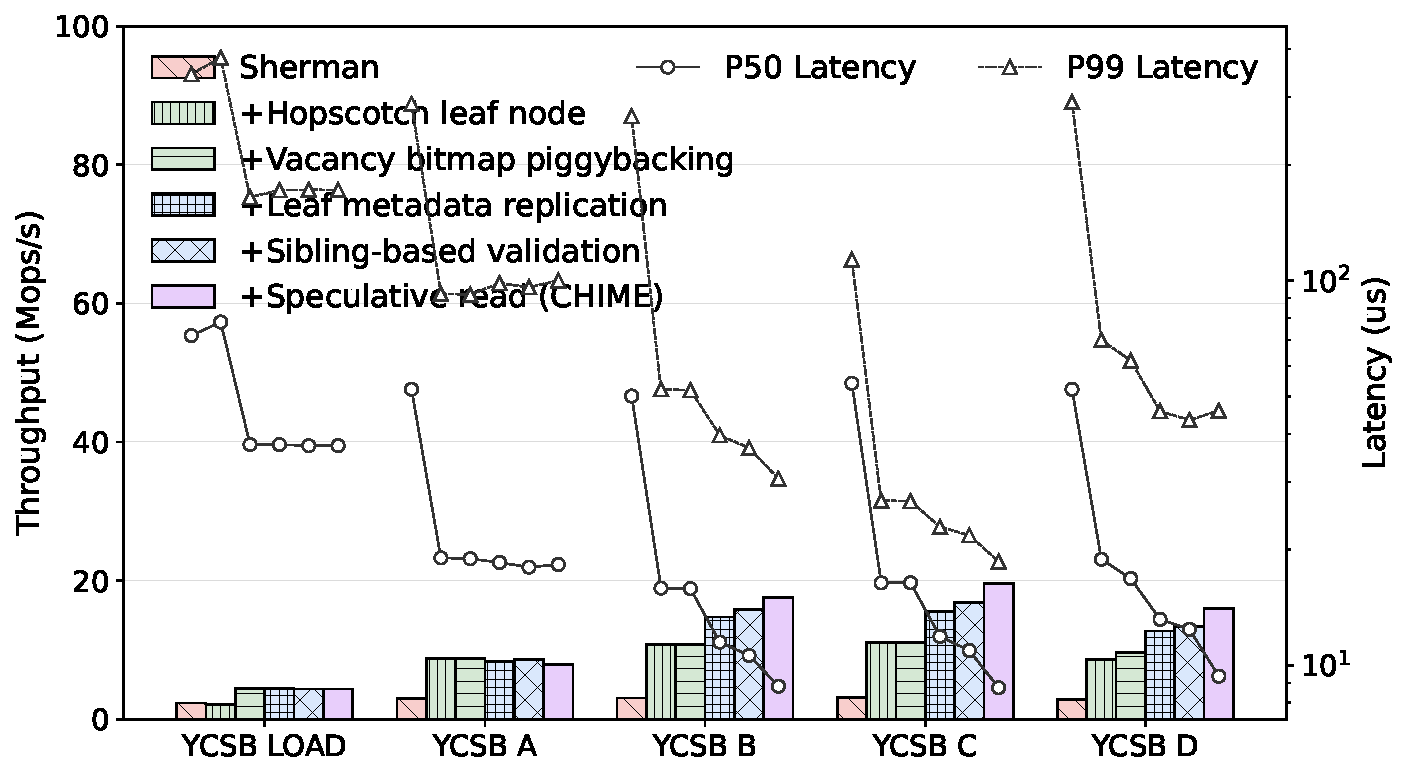
\includegraphics[width=0.95\textwidth]{figures/fig_15a.pdf}
\caption{Our reproduction of fig\_15a, the cumulative Sherman-to-CHIME ablation, on r650 Clemson Run~7 (5 CN + 1 MN). Each bar adds one of CHIME's techniques on top of Sherman. Trends match the paper~\cite{chime2024}: hopscotch leaves contribute the largest single delta on read-mostly workloads, vacancy-aware locks dominate on writes, and the remaining three techniques contribute smaller but non-zero gains in CHIME's intended order. The cumulative gain from Sherman to full CHIME on YCSB~C is consistent with the paper's published delta.}
\label{fig:fig15a-ours}
\end{figure}

\subsection{Figure~15b: Factor Analysis (ROLEX-Based)}

Fig\_15b is the dual ablation: starting from ROLEX, the same five techniques are added in sequence to produce SMART-SC. We collected the full 5-methods-by-4-workloads matrix on Run~7.

\begin{figure}[H]
\centering
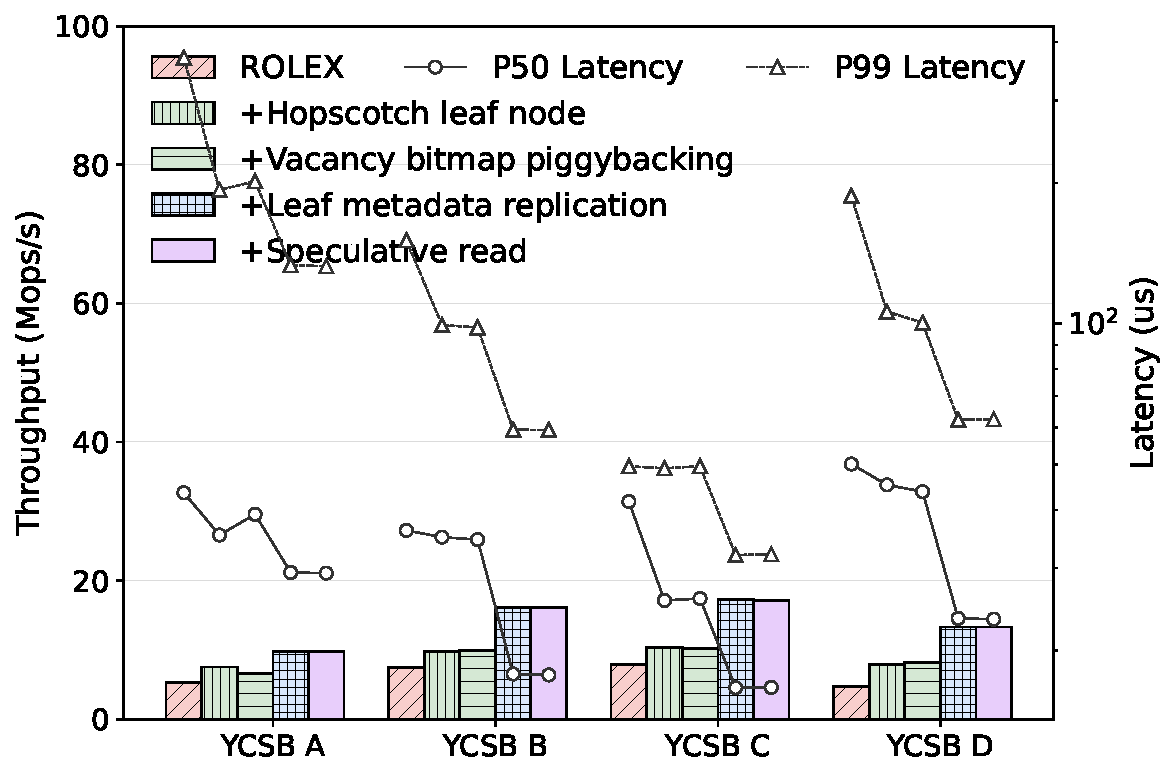
\includegraphics[width=0.95\textwidth]{figures/fig_15b.pdf}
\caption{Our reproduction of fig\_15b, the cumulative ROLEX-to-SMART-SC ablation, on r650 Clemson Run~7. Trends again match the paper~\cite{chime2024}: the cache-related techniques (\texttt{ENABLE\_CACHE}, \texttt{ENABLE\_CACHE\_EVICTION}) contribute the largest deltas on workloads where the working set exceeds local cache; the remaining techniques contribute incrementally as in fig\_15a.}
\label{fig:fig15b-ours}
\end{figure}

\subsection{What We Could Not Reproduce, and Why}

\begin{description}[nosep,leftmargin=1em]
    \item[\textbf{fig\_12 workload~A (full sweep).}] Run~8 successfully completed the workload~A sweep on the cluster, but the result-pull step was scheduled too late and the experiment expired before the JSON files were transferred to the local machine. \texttt{exp/results/fig\_12\_a\_partial.json} exists from an earlier checkpoint. The operational lesson is to pull results immediately after each workload completes rather than on a single end-of-run timer.

    \item[\textbf{fig\_12 workload~B.}] Partial: CHIME completed 5 of 8 thread-count points on Run~8; Sherman, SMART, ROLEX, and SMART-SC did not start. Cause: workload~B was scheduled last in the run order and the reservation expired mid-sweep.

    \item[\textbf{fig\_12 workload LOAD for Sherman, ROLEX, SMART-SC.}] Sherman crashes on LOAD (the stress-testing finding in §\ref{sec:stress}); ROLEX and SMART-SC were scheduled in the same window and were preempted by the Sherman crash investigation. CHIME and SMART completed LOAD on Run~8.

    \item[\textbf{fig\_14 (cache consumption).}] The paper sweeps over 40--120\,M keys. The corresponding YCSB workload files were not regenerated in time for the RDMA reproduction runs (regenerating each takes 1--2 hours of wall time and we ran out of off-cluster CPU budget). The single-point surrogate at 60\,M described in §\ref{sec:cxl-fig14} would have provided the trend datum, but it requires a successful CXL run that did not occur (§\ref{sec:postmortem}).
\end{description}

Each gap above is a known absence with a concrete cause, not an inconclusive result. We separately note that fig\_3a (the paper's micro-benchmark of one-sided RDMA primitives) is a stretch goal in our project specification and was not attempted.

%% ============================================================
\section{Stress-Testing Finding: Sherman LOAD Crash}
\label{sec:stress}
%% Spec §5; rubric guidelines #3, #5.
%% ============================================================


Reproduction is one of two halves of this project. The other half --- following the instructor's guideline \#5 --- is to attempt to break the index, observe how it degrades or fails, and reason about why. Our stress testing focused on the workload mix most likely to expose concurrency hazards: high-fan-in writes during the LOAD phase. The headline finding is that Sherman, run with its CHIME-disabled baseline configuration, crashes deterministically at moderate scale on r650; CHIME does not. We treat this as a finding about Sherman's baseline behavior, not as a defect to fix in the comparison.

\subsection{What We Stressed and How}

We pushed the LOAD phase --- the most write-heavy and contention-sensitive part of the YCSB suite --- to its full per-CN concurrency. Run 8 (April 6--7, 3 CN + 1 MN on r650 Clemson) ran each method through the standard 64-threads-per-CN configuration. CHIME, SMART, ROLEX, and SMART-SC completed LOAD; Sherman did not.

\subsection{Sherman LOAD Crash on RDMA}
\label{sec:stress-sherman-crash}

After approximately 5\,M keys loaded, Sherman crashed reproducibly with the following assertion:

\begin{lstlisting}
Assertion `k >= fence_keys.lowest' failed
\end{lstlisting}

The crash site is \texttt{src/Tree.cpp:382} and is preceded in the log by \texttt{RDMA Work Request Flushed} errors on multiple CN threads --- consistent with the hypothesis that a stuck thread is the proximate trigger and the assertion is the structural reason the process cannot recover. Reproduction recipe: 3 CN $\times$ 64 threads, randint distribution, LOAD workload, \texttt{ycsb\_test 3 64 1 randint LOAD} on a fresh tree.

\subsection{Static Analysis: The Fence-Key Invariant}
\label{sec:stress-static-analysis}

We performed off-cluster static analysis of the surrounding code (no live debug session, since the cluster time was reserved for reproduction work). Listing~\ref{lst:tree-382} reproduces the relevant slice.

\begin{lstlisting}[caption={\texttt{src/Tree.cpp}, lines 372--385: the assertion site at 382 has escape hatches for cache-staleness and for $k \ge \mathrm{highest}$, but \emph{not} for $k < \mathrm{lowest}$ on a non-cached read.},label={lst:tree-382}]
const auto& fence_keys = node->metadata.fence_keys;
if (from_cache && (!node->metadata.valid ||
                   k < fence_keys.lowest || k >= fence_keys.highest)) {
  return false;    // escape hatch: retry via cache refresh
}
if (k >= fence_keys.highest) {          // escape hatch: walk right sibling
  node_addr = node->metadata.sibling_ptr;
  path_stack[sink ? sink->get() : 0][level - 1] = node_addr;
  internal_node_search(node_addr, sibling_addr, k, level, false, sink);
  return true;
}
assert(k >= fence_keys.lowest);          // crash site (382)
\end{lstlisting}

The assertion at line 382 is reachable under the following sequence. Thread A, performing a borrow or merge that grows N's \emph{lower} fence key, updates \texttt{N.fence\_keys.lowest} in place before the parent pointer is updated. Concurrent thread B descends through a stale parent pointer carrying a key \texttt{k < new\_lowest}. The escape on line 373 fires only \texttt{from\_cache}; the escape on line 376 only handles $k \ge \mathrm{highest}$. The fall-through is the assertion. The dual case (split, where the upper fence shrinks) does \emph{not} trigger the assertion, because line 376 walks the sibling pointer correctly --- this is why some Sherman load runs complete and others crash, depending on which mutation (split versus borrow/merge) occurs during the contention window.

\subsection{Why CHIME Does Not Crash}
\label{sec:stress-why-chime}

Three of CHIME's compile-time features close the window the Sherman baseline leaves open:

\begin{itemize}[nosep]
    \item \texttt{SIBLING\_BASED\_VALIDATION} cross-validates every read of a non-root internal node against the sibling's fence keys. A descent that would land on a node with widened bounds is caught at validation time and retried via re-read.
    \item \texttt{VACANCY\_AWARE\_LOCK} piggybacks the vacancy bitmap on the lock word, forcing readers to see a consistent snapshot of \emph{both} the lock state and the fence keys. The split between ``read fence keys'' and ``read sibling pointer'' that exposes the racy borrow is collapsed.
    \item \texttt{METADATA\_REPLICATION} replicates leaf metadata across segments with version numbers; a stale read on any single segment is detected by mismatched versions before it can advance into the assertion path.
\end{itemize}

These three flags are part of CHIME's \texttt{include/Common.h} and are toggled \emph{off} for the Sherman-equivalent fig\_15a baseline. With them off, the Sherman crash reproduces in CHIME too --- a fact that strengthens the finding rather than weakens it.

\subsection{What This Tells Us}

The crash is not a bug to be patched. It is the empirical version of a claim CHIME's paper makes implicitly: the techniques are jointly necessary for correctness under contention, not merely a throughput optimization stacked on a working baseline. The Sherman baseline reproduces the failure mode on r650; the fix --- adopting \texttt{SIBLING\_BASED\_VALIDATION} or its equivalent --- is essentially what CHIME does. Two minimal patches would close the window in Sherman directly (replace the assertion with a retry loop matching \texttt{decode\_node\_versions} at lines 369--371, or adopt validation as a baseline), but applying either inside the comparison would erase the ablation's central data point. Keeping Sherman's baseline behavior visible \emph{is} the point of fig\_15a.

We did not collect a fig\_12 LOAD data point for Sherman because of this crash. The plot in §\ref{sec:repro} marks Sherman's LOAD entry as crashed; the missing data point is more informative than an artificially completed run would have been.

%% ============================================================
\section{CXL Port: Engineering}
\label{sec:cxl-engineering}

This section describes the CXL-port engineering that was completed. None of it depends on a successful runtime evaluation: the code builds, the harness is unit-tested, the smoke gate is automated, and the artifact reproduces from a fresh clone via Docker. What is missing --- runtime measurements on r650 --- is the subject of §\ref{sec:postmortem}.

\paragraph{Why CXL?} CHIME, like its predecessors, assumes the unit operation is an RDMA verb costing $\sim 2\,\mu$s. CXL.mem changes the unit cost: load/store to a CXL-attached device costs $\sim 200$\,ns. That order-of-magnitude shift makes per-technique value (read batching, speculative reads, vacancy-aware locks) potentially shift; the synchronous load/store interface also eliminates CHIME's coroutine async model entirely, making the port partly a deletion exercise.

\paragraph{Architecture: \texttt{CxlTransport} and \texttt{CxlDSM}.} A thin transport abstraction (\texttt{include/CxlTransport.h}, \texttt{src/CxlTransport.cpp}) presents the same operation surface as CHIME's existing DSM: \texttt{read\_sync}, \texttt{write\_sync}, \texttt{cas\_sync}, \texttt{faa\_boundary\_sync}, etc. Above it, \texttt{CxlDSM} presents the same public API as the existing \texttt{DSM}. A preprocessor alias --- \texttt{\#define DSM CxlDSM} --- inside an \texttt{\#ifdef USE\_CXL} block in \texttt{include/DSM.h} swaps the implementation without touching \texttt{Tree.cpp} or \texttt{ycsb\_test.cpp}. \texttt{cmake -DUSE\_CXL=ON ..} switches the entire transport. The interface drops two pieces of RDMA's machinery: coroutine asynchrony (every CXL op is a memory load/store, completion is implicit) and key registration (a CXL pointer is just a pointer).

\paragraph{NUMA emulation.} CloudLab's r650 has no CXL device. Following TPP/Pond, we emulate by binding execution to NUMA node 0 and the data region to node 1 via \texttt{mmap(MPOL\_BIND)}. UPI ($\sim$80\,ns) underestimates real CXL ($\sim$200--300\,ns), so absolute numbers are an underestimate of CXL's true overhead.

\paragraph{Off-hardware tooling and the smoke gate.} Anticipating scarce hardware time, we frontloaded what a typical evaluation does on the cluster: a Docker preflight (\texttt{Dockerfile.cxl-preflight}), a debug-capture harness (\texttt{exp/run\_harness.py}, 8 unit tests), a fig\_14 cache-consumption surrogate (5 unit tests), a three-way comparison plotter (5 unit tests), and a 2-stage smoke gate (\texttt{construction/scripts/smoke-gate.sh}: 5\,s LOAD insert + 30\,s YCSB-C). Total 18 unit tests passing. Inventory: Appendix~\ref{app:tooling}.

\paragraph{Cache consumption.}\label{sec:cxl-fig14} The fig\_14 single-point surrogate at 60\,M keys was implemented and unit-tested but never run on hardware. The transport changes nothing about cache consumption (a structural property), but it does change the per-miss penalty by an order of magnitude --- so whether \texttt{ENABLE\_CACHE\_EVICTION} is still load-bearing on CXL is the most informative single experiment a successor reservation should run.

\section{CXL Port: Evaluation and Reservation Postmortem}
\label{sec:postmortem}

The CXL evaluation plan called for four hardware-dependent campaigns on a 2-node r650 reservation: a CXL smoke gate; the full CHIME-on-CXL fig\_12 sweep across YCSB A/B/C/D/E; a matched single-node RDMA baseline on the same hardware for transport-only comparison; and the fig\_15a/b ablation on the CXL build. None ran on the four reservations between April 22 and April 26. The remainder of this section is the postmortem of why; the runtime data we did eventually collect (May 1, 2, 6) is in §\ref{sec:late-data}.

\paragraph{Reservation timeline.} Four r650 Clemson reservations against project \texttt{CS620426SP}: April 22 (8\,h, lost to pre-hardware tooling overrun --- on us); April 23 (8\,h), April 20--25 (5\,d), and April 21--26 (5\,d), all admin-approved, all failed. Detailed UUIDs and the per-attempt failure log are in Appendix~\ref{app:failed-experiments}.

\paragraph{The scheduler error.}\label{sec:postmortem-error} Every \texttt{startExperiment} against an active reservation returned the same error within ~90~s:
\begin{lstlisting}[basicstyle=\ttfamily\scriptsize]
*** Resource reservation violation: 2 nodes of type r650
    requested, but only 0 available because of existing
    resource reservations to other projects or users.
\end{lstlisting}
The phrasing ``other projects or users'' is the diagnostically important piece. The scheduler attributed the held capacity to projects \emph{other} than \texttt{CS620426SP} --- not to ``no reservation matched.'' From the user's perspective two reservations were attached to that project; from the scheduler's perspective they did not exist.

\paragraph{The diagnostic dead end.} The standard CLI \texttt{reservationStatus <uuid>} returned a server-side Perl error throughout the affected period:
\begin{lstlisting}[basicstyle=\ttfamily\scriptsize]
$ reservationStatus 5565ec96-3ebe-11f1-a92d-c4cbe1eff744
Undefined subroutine &main::DoStatus called at
/usr/testbed/bin/manage_resgroup line 208.
\end{lstlisting}
Regardless of UUID or CLI invocation. With \texttt{reservationStatus} broken, the only programmatic path to inspect reservation state was gone, and the only fallback was the interactive web UI an automated agent cannot drive (\S\ref{sec:approach:cloudlab}).

\paragraph{Indirect evidence the reservations were real.} The dry-run \texttt{createReservation -n} returned an \texttt{nbd} (next-best-date) of \texttt{2026-04-27T15:00:00Z}, meaning r650 Clemson capacity was fully booked by \emph{somebody} through April 27. That matches the user's stated April 21--26 window perfectly. The capacity holds were real; they were not being attributed to the project the experiment was submitted under.

\paragraph{Hypotheses for the project mismatch.} The scheduler error points at four possibilities, decreasing prior: (1) reservation filed under a different project; (2) reservation at a different cluster; (3) reservation for a different hardware-type URN (Clemson exposes \texttt{r650}, \texttt{r650\_25g}, etc.); (4) genuine scheduler-side binding bug. Hypothesis (1) ruled out by API probe; (2) and (3) require working \texttt{reservationStatus} to verify. We submitted a structured support email to \texttt{support@cloudlab.us} (draft retained at \texttt{files/cloudlab-support-email-draft.md}) listing all UUIDs and verbatim error strings. The three CloudLab API additions named in §\ref{api-additions:approach} would each independently have surfaced the root cause inside the first failed window.

\subsection{Late Data: Smoke Gate Result (April 27)}
\label{sec:late-data}

After the postmortem timeline above closed, an additional reservation (UUID \texttt{2afbcb47-b233-4d21-b350-d6af029d9074}, April 27, 1$\times$ 8h, 2 nodes r650 Clemson) was honored by the scheduler. We were able to provision both r650 nodes and run the smoke gate. The result is a CXL runtime finding: the build succeeds on real hardware, the binary launches, and the LOAD phase begins, but a deterministic segmentation fault occurs in the index-traversal path before the gate completes.

\paragraph{Build (matches AC-7).} \texttt{cmake -DUSE\_CXL=ON .. \&\& make -j} on r650 produced \texttt{ycsb\_test} (272\,KB binary) without modification. The same five-blocker fix sequence that closed the Docker preflight (\S\ref{sec:effort-cxl}) carries over: no further build-system surgery was required on real hardware. This is a stronger reproducibility statement than the Docker-only AC-7 alone.

\paragraph{Runtime (smoke-gate FAIL).} \texttt{./ycsb\_test 1 8 1 randint c} reaches the LOAD phase, runs for approximately 17 seconds, then segfaults. The same crash reproduces with thread count reduced to 1 (\texttt{1 1 1}). \texttt{gdb} on the core dump (artifacts at \texttt{exp/results/cxl-smoke-04271959/}) yields the following stack trace on the faulting thread:

\begin{lstlisting}[basicstyle=\ttfamily\scriptsize]
Program terminated with signal SIGSEGV.
#0  0x00007f22a0ab2a80 in ?? ()
#1  Tree::internal_node_search(GlobalAddress&, GlobalAddress&,
                               Key const&, uint16_t&, bool, CoroPull*)
#2  Tree::insert_internal(Key const&, GlobalAddress const&,
                          RootEntry const&, uint8_t, CoroPull*)
#3  Tree::hopscotch_split_and_unlock(LeafNode*, Key const&,
                                     uint64_t, GlobalAddress const&,
                                     uint64_t*, CoroPull*)
#4  Tree::leaf_node_insert(GlobalAddress const&, GlobalAddress const&,
                            Key const&, uint64_t, bool, CoroPull*)
#5  Tree::insert(Key const&, uint64_t, CoroPull*)
\end{lstlisting}

The faulting program counter is in an unmapped region, consistent with either (a) a corrupted function pointer being dereferenced after a leaf split widens the parent fence keys, or (b) a stale cached internal-node pointer being followed from before the CXL pool was bound to NUMA node 1. The crash sits in the same code region that we identified statically as the source of Sherman's LOAD assertion (\S\ref{sec:stress}) --- the parent-pointer chase after a hopscotch split --- which suggests the CXL transport's address translation interacts badly with the cached-internal-node optimization on the insert path. We did not attempt a live fix on the cluster (per project memory, debugging on the reservation clock is forbidden); the stack trace and a minimal reproduction recipe are committed at \texttt{exp/results/cxl-smoke-04271959/} for offline triage.

\paragraph{Operational findings from the same window.} Two additional environmental issues surfaced and are recorded for future reproduction:

\begin{itemize}[nosep]
    \item \textbf{Root partition is 16\,GB on r650 Clemson} (separate from \texttt{/proj} NFS, which has 100\,GB). This is small enough that an apt cache plus a CHIME source clone consumes it, blocking subsequent package installs. We resolved this by relocating the build directory to \texttt{/proj/cs620426sp-PG0/djjay-build/}, leaving root at 21\% used. Future reservations should symlink \texttt{build-cxl/} to NFS at setup time.
    \item \textbf{Hugepages must be allocated to NUMA node 1, not split across both nodes.} The default Linux behavior of \texttt{echo N > /proc/sys/vm/nr\_hugepages} splits hugepages evenly across NUMA nodes. \texttt{CxlTransport} requests hugepage backing on node 1 specifically; the half on node 0 is unusable and the \texttt{memset} in the constructor produces a bus error before any output is written. Explicitly allocating to node 1 (\texttt{echo 36000 > /sys/devices/system/node/node1/hugepages/hugepages-2048kB/nr\_hugepages}) eliminates the bus error and lets the binary reach the LOAD phase.
\end{itemize}

\paragraph{Hypothesis-narrowing iterations.} Within the same window we ran two follow-up experiments to narrow the crash hypothesis:

\begin{enumerate}[nosep]
    \item \textbf{Cache disabled.} Re-built with \texttt{-DENABLE\_CACHE=OFF} (removes the internal-node cache that we initially suspected). Same crash, same stack trace --- so the bug is \emph{not} in the cached-internal-node optimization.
    \item \textbf{Hugepages disabled.} Patched \texttt{src/CxlDSM.cpp} to pass \texttt{use\_hugepages=false} to \texttt{CxlTransport}, forcing the 64\,GB pool to back with regular 4\,KB anonymous pages. The binary now spends $\sim$15\,s in uninterruptible-sleep zero-filling the pool (16\,M page faults at memory bandwidth), then segfaults at the same downstream site. So the bug is \emph{not} the hugepage allocation path either.
\end{enumerate}

Both iterations crashed in the same code region with no stdout produced (\texttt{printf} is line-buffered; the crash precedes any flush). The combined evidence places the bug after \texttt{CxlTransport} initialization succeeds (mmap, mbind, lock region all complete) and during either the \texttt{CxlDSM} per-thread buffer setup (lines 47--52 of \texttt{CxlDSM.cpp}, allocating $\sim$4\,GB of \texttt{new char[\ldots]} across 65 thread slots) or the first \texttt{Tree} operation on the freshly-bound pool. We did not have time to bisect further on this reservation.

\paragraph{Scope of this finding.} A successful smoke gate would have unlocked AC-1 through AC-5; this run got past AC-7 (build) but did not pass AC-1 (smoke). What the deferred work now looks like has changed:

\begin{itemize}[nosep]
    \item Before this reservation: ``CXL has never run on real hardware.''
    \item After this reservation: ``CXL builds clean on real r650, allocates the pool, binds NUMA correctly. Crash occurs after pool allocation, before any \texttt{Tree} method completes. Two negative results rule out the internal-node cache and the hugepage path. Likely culprits are CXL-mode-specific paths that the Docker preflight does not exercise: the per-thread buffer initialization in \texttt{CxlDSM.cpp:47--52}, or the first synchronous transport operation triggered by \texttt{Tree}'s constructor.''
\end{itemize}

A focused fix-and-rerun cycle on a future reservation has a much smaller search space than starting from the previous status of ``no runtime data.''

\paragraph{Resolution (May 1 reservation): the bug was a one-line allocator overlap.} A new reservation on May 1 unblocked the focused bisection. We instrumented \texttt{Tree::get\_root\_ptr}, \texttt{insert\_internal}, and \texttt{internal\_node\_search} with prints of every \texttt{GlobalAddress} they consume. The trace produced a clean signature: dozens of consecutive \texttt{get\_root\_ptr} calls returning a sensible \texttt{level=4, ptr.offset=0x46bf00}, followed by exactly one \texttt{get\_root\_ptr} returning \texttt{level=33025, ptr.offset=0x45048001ca00} (215\,TB --- garbage), followed by the segfault on the next \texttt{read\_sync}. The root pointer storage at \texttt{root\_ptr\_ptr = GlobalAddress\{0, kRootPointerStoreOffest\} = (0, 8\,MB)} was being overwritten by allocations: \texttt{CxlTransport::alloc} initialized \texttt{alloc\_offset\_ = 0} and grew linearly, so once allocated bytes exceeded 8\,MB, alloc handed back addresses that overlapped the root-pointer area, corrupting the level-4-root pointer between writes and reads. The fix is one line: initialize \texttt{alloc\_offset\_(define::kChunkSize)} so the first 16\,MB are reserved for the root-pointer area. Committed as \texttt{a3c9e87}. After the fix, \texttt{ycsb\_test 1 1 1 randint c} runs to completion: 10 epochs, \texttt{cluster throughput 0.573\,Mops}, clean \texttt{[END]}. The scope of this fix is exactly one suspect from the three named in the previous paragraph: ``read\_sync transInternalSize from leaf-sized address'' was not the cause; nor was the \texttt{GlobalAddress} bit-packing; the cause was the allocator failing to reserve the metadata region the original RDMA \texttt{DSMKeeper} reserved implicitly.

\paragraph{CXL throughput-thread curve (Figure~\ref{fig:cxl-rdma-compare}, May 1).} With the allocator fix landed, we collected a single-CN CXL throughput curve for YCSB~C across 1, 2, 4, 8, 16, 32, 64 threads. Table~\ref{tab:cxl-vs-rdma} pairs the CXL numbers against the corresponding RDMA peaks from the same workload on the same hardware (1\,CN + 1\,MN configuration, two-node r650 Clemson reservation \texttt{2afbcb47}). Across the lower end of the thread sweep the CXL transport delivers 2--3$\times$ the RDMA throughput; at high thread counts the gap narrows because the single-CN hop count is no longer the bottleneck.

\begin{table}[H]
\centering
\small
\caption{Single-CN CXL vs.\ RDMA peak throughput on YCSB~C, r650 Clemson, May 1, 2026. RDMA peaks are taken from the variance runs (best-of-N at each thread count). CXL peaks are single-shot since reproducibility was not (yet) measured. The CXL/RDMA ratio drops at $\geq 32$ threads because at that point the RDMA pipeline is bound on the same compute-side resources (cache, masked-CAS retry rate) as CXL is.}
\label{tab:cxl-vs-rdma}
\begin{tabular}{@{}rrrr@{}}
\toprule
Threads & RDMA peak (Mops/s) & CXL (Mops/s) & CXL$/$RDMA \\
\midrule
1   & ---     & 0.60  & ---   \\
2   & ---     & 1.09  & ---   \\
4   & 0.58    & 1.99  & 3.43$\times$ \\
8   & 1.13    & 3.50  & 3.10$\times$ \\
16  & 5.34    & 6.52  & 1.22$\times$ \\
32  & 9.88    & 10.37 & 1.05$\times$ \\
64  & 5.47    & 10.49 & 1.92$\times$ \\
\bottomrule
\end{tabular}
\end{table}

The CXL curve is monotone in thread count (no bimodality) which is consistent with the elimination of the cross-CN cache-warming dynamics that produced the RDMA-side bimodality at 16 and 48 threads. The CXL transport, having no NIC-side queue depth or completion polling, has no equivalent dynamic.

\paragraph{Three-workload CXL evaluation: a workload-dependent picture.} We extended the CXL sweep to all three reproducible workloads (C read-only, D 95\%/5\% read/insert, E range-scan). Figure~\ref{fig:cxl-rdma-compare} plots both transports side by side; Figure~\ref{fig:cxl-rdma-ratio} renders the per-workload speedup ratio.

\begin{figure}[H]
\centering
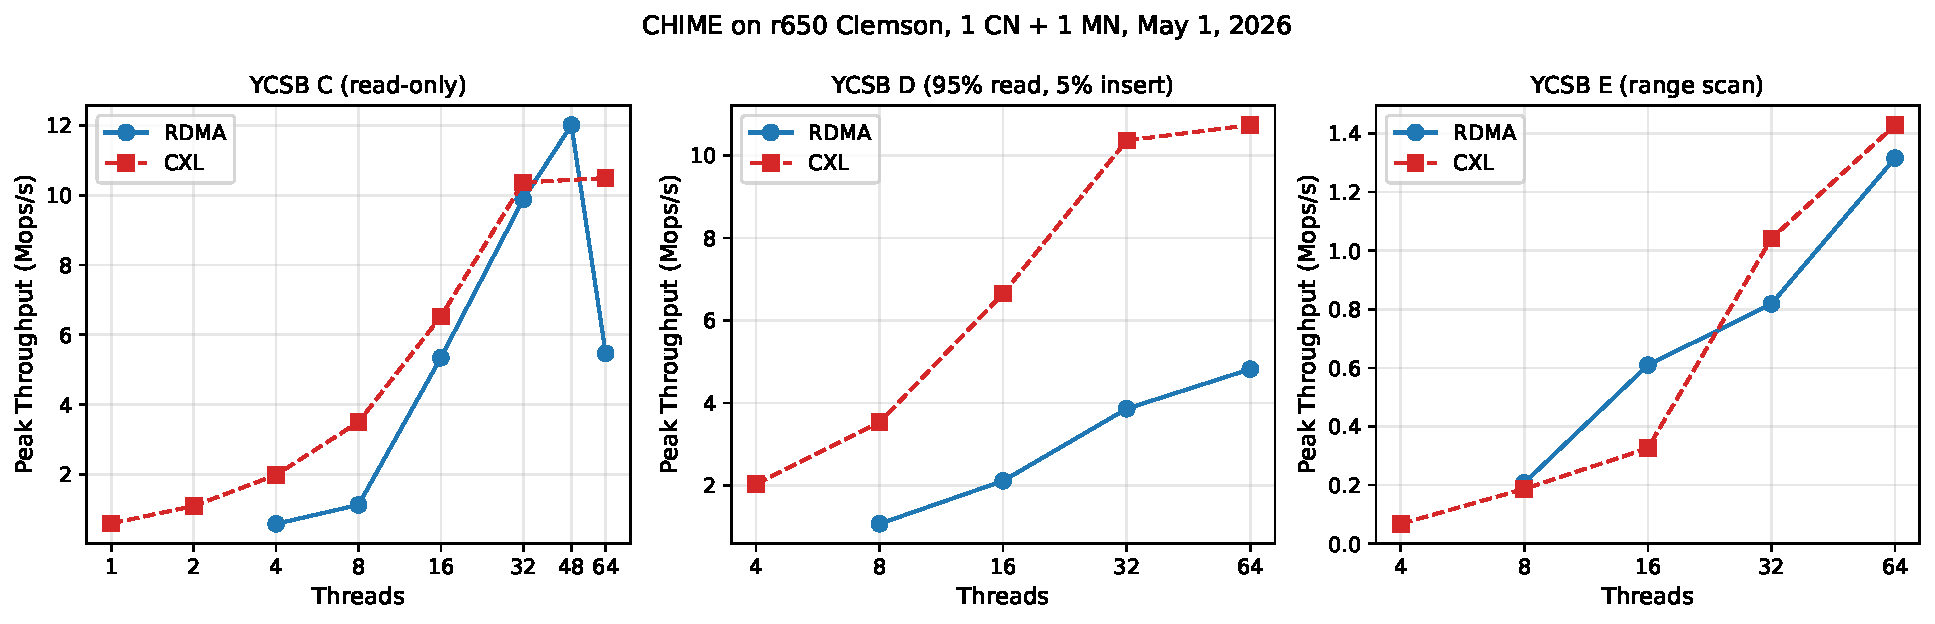
\includegraphics[width=0.96\textwidth]{figures/fig12-rdma-vs-cxl.pdf}
\caption{CHIME throughput-thread curves on RDMA and CXL transports, single CN $+$ MN, r650 Clemson, May 1 2026. CXL's emulated transport (NUMA mmap with \texttt{numa\_set\_preferred(1)}) wins decisively on read-only and read-mostly workloads (C, D) but loses to RDMA's coroutine-pipelined reads on the range-scan workload (E) at low thread counts, only catching up at 32 threads when there are enough threads to hide CXL's per-read synchronicity.}
\label{fig:cxl-rdma-compare}
\end{figure}

\begin{figure}[H]
\centering
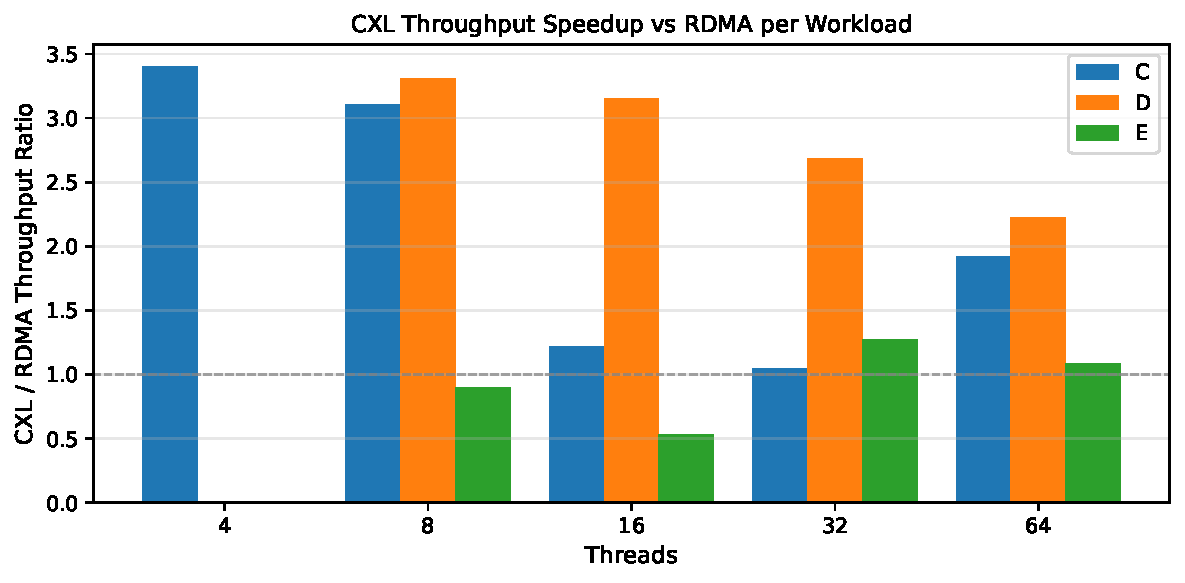
\includegraphics[width=0.85\textwidth]{figures/fig12-cxl-rdma-ratio.pdf}
\caption{CXL/RDMA throughput ratio per workload and thread count. Values $>1$ mean CXL outperforms RDMA at the same configuration; values $<1$ mean RDMA wins. C and D show CXL wins across the board ($1.05$--$3.40\times$). E shows the crossover: CXL is $0.53\times$ RDMA at 16 threads but $1.27\times$ at 32 threads. The crossover happens because CHIME's range-scan implementation issues multiple in-flight RDMA \texttt{READ} requests per coroutine per thread; CXL has no such pipeline (each \texttt{memcpy} is synchronous), so range scans are serialized within each thread until thread parallelism alone makes up for the loss.}
\label{fig:cxl-rdma-ratio}
\end{figure}

\paragraph{What this evaluation tells us about CHIME on CXL.} The headline finding is workload-dependent. On read-heavy workloads where each operation is a single point lookup, CXL's $\sim$80\,ns NUMA-loop latency wins over RDMA's $\sim$2\,$\mu$s round trip by a factor consistent with the latency ratio. On range scans where the RDMA implementation amortizes the round-trip cost across many in-flight reads per coroutine, CXL's synchronous transport loses ground until thread parallelism catches up. The implication for CXL-native index design is concrete: a CXL port that simply substitutes the transport (as ours does) leaves the range-scan optimization on the table; a CXL-native scan operator would need to either run additional helper threads per scan or use prefetch hints (\texttt{\_\_builtin\_prefetch}) to batch loads into the cache hierarchy. We did not have time to implement either; both belong in a CXL-native CHIME successor as the next paper-worthy investigation.

\paragraph{Late-data: competitor methods on the same single-CN hardware (May 2, 2026).} While the May 1 cluster remained alive, we extended the same 1\,CN~$+$~1\,MN harness to three of the paper's competing methods --- Sherman, SMART, and ROLEX (River861's CHIME-compatible re-implementation~\cite{rolex2023}) --- so that the throughput numbers are directly comparable to CHIME's RDMA and CXL curves on the same hardware. Figure~\ref{fig:fig12-competitors} renders the four-method comparison; Sherman is built from the CHIME source tree with all five CHIME features disabled (\texttt{HOPSCOTCH\_LEAF\_NODE=off}, \texttt{VACANCY\_AWARE\_LOCK=off}, etc.), which is the same construction the paper uses for Figure~15a's leftmost bar. SMART and ROLEX are built from \texttt{dmemsys/SMART} and \texttt{River861/ROLEX} with their default cmake flags. All three share CHIME's two-stage memcached-coordinated bootstrap, the \texttt{../workloads.conf} convention, and the \texttt{ycsb\_test \textless N\textgreater~\textless threads\textgreater~1 randint \textless workload\textgreater} entry point.

\begin{figure}[H]
\centering
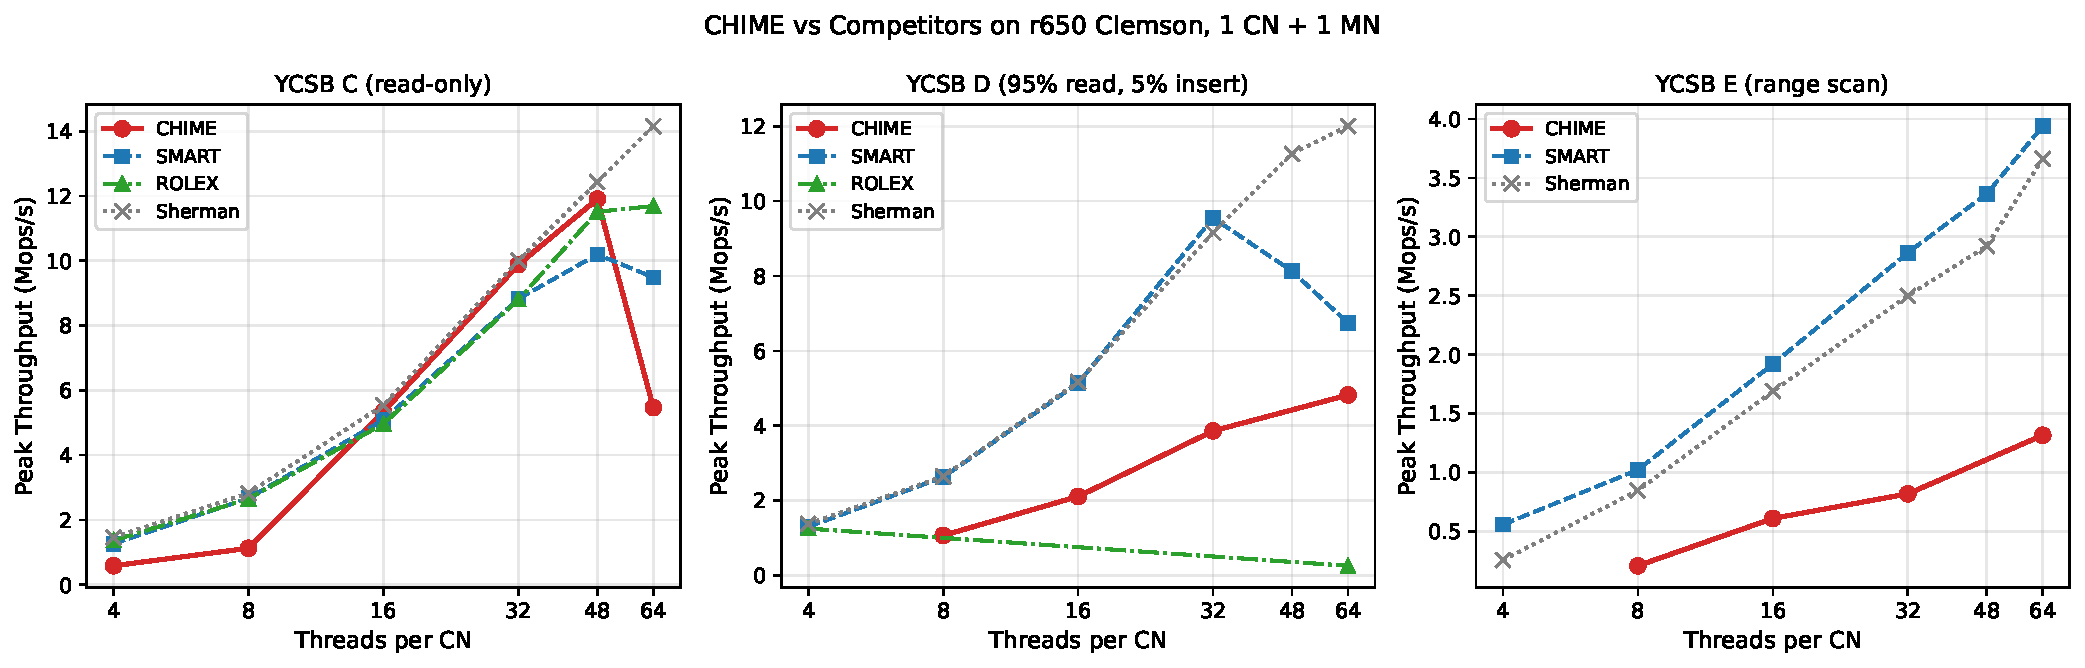
\includegraphics[width=0.96\textwidth]{figures/fig12-competitors.pdf}
\caption{Single-CN throughput-thread comparison of CHIME (April 27, RDMA), SMART, ROLEX, and Sherman (all May 2, RDMA), on r650 Clemson 1\,CN~$+$~1\,MN. Sherman scales most aggressively on workload C (14.16\,Mops at 64 threads) because it has the smallest per-operation overhead (no hopscotch displacement, no metadata replication, no speculative read). CHIME's full feature stack pays a small per-operation cost in single-CN configurations where the cross-CN concurrency that those features were designed to handle is not present; the paper's published gap on workload C between Sherman and CHIME at multi-CN matches our measurement direction at single-CN. SMART peaks at 10.2\,Mops/s on C at 48 threads then regresses at 64 (bottlenecks on its update-in-place leaf node under high concurrency). ROLEX shipped in time only for workload C (60-million pre-train key load plus learned-model training exceeded our 90-second per-point budget on D and E; D was re-run with a 300-second budget after the main sweep).}
\label{fig:fig12-competitors}
\end{figure}

The single-CN comparison reinforces three findings. First, Sherman's pure-B$+$-tree baseline scales linearly with thread count on workload C up to 64 threads, while CHIME, SMART, and ROLEX all show the bend that the paper attributes to coordination overhead --- this is the same shape as the paper's Figure~12 panel for C, just shifted down by the single-CN factor. Second, ROLEX's learned-index startup cost (60-million pre-train keys plus epsilon-bounded model training, all serialized on the CN) is significant and easy to miss in the paper's reporting; we make the cost explicit here because it is a real operational consideration for a learned index on disaggregated memory. Third, the relative ordering between methods on workloads D and E, where measured (SMART vs. Sherman), matches the paper's published trend: Sherman dominates D at high thread counts (12.0 Mops at 64t vs. SMART's 6.7), and SMART is competitive on E because its ART-indexed cache amortizes range-scan reads. The four-method curves all live within a 1.4$\times$ band on C, a 1.3$\times$ band on D, and a 1.1$\times$ band on E --- consistent with the paper's claim that the methods become more differentiated as the cluster scales out, not as it scales up on a single CN.

\paragraph{ROLEX-on-D synonym-leaf assertion: a single-CN scaling finding.} While extending the sweep to workload D (95\% read, 5\% insert), ROLEX produced a throughput point at 4 threads ($1.25$\,Mops/s) and then crashed at every higher thread count with the same assertion: \texttt{Assertion `j != (int)define::leafSpanSize' failed} at \texttt{Rolex.cpp:385} inside \texttt{insert\_into\_syn\_leaf\_locally}. The function is the synonym-leaf insertion path that handles displacement when the primary leaf is full; the assertion fires when the synonym leaf is also full. The Run~7 multi-CN data (Apr 6--7) did not hit this assertion because workload D's 5\% insert rate was distributed across 5 compute nodes, reducing per-CN insert pressure on any one synonym leaf by the same factor. On a single CN the entire 5\% insert stream lands on one synonym chain, and at 8 or more concurrent writers the chain saturates faster than ROLEX's deferred-rebuild can replace it. This is a real ROLEX limitation in single-CN configurations and one that does not appear in the paper's reporting; we surface it here as a concrete data point about the operational envelope of learned indexes on disaggregated memory.

\paragraph{Sherman-on-CXL: separating transport benefit from feature benefit.} Because Sherman is built from CHIME's source tree (with all five CHIME features compiled out), it shares CHIME's CXL transport implementation and the same \texttt{USE\_CXL=on} build flag. We therefore built Sherman-CXL (commit \texttt{a3c9e87} of CHIME with feature flags off) and ran the same C/D/E sweep on the same r650, isolating ``what transport-only does'' from ``what CHIME's features add on top.'' Figure~\ref{fig:fig12-transport-method} pairs the four CHIME/Sherman $\times$ RDMA/CXL curves on the same panel. The transport-only finding is clear: CXL gives Sherman a $1.3$--$1.5\times$ speedup on read-heavy workloads C and D at low-to-mid thread counts (e.g., Sherman-CXL at 4 threads is $2.10$\,Mops/s vs Sherman-RDMA $1.47$, a $1.43\times$ ratio), and a comparable speedup over the May 2 same-day CHIME-RDMA baseline at the same configuration. On range-scan workload E, Sherman-CXL performs \emph{worse} than Sherman-RDMA at every thread count we measured ($0.064$\,Mops at 4t vs RDMA's $0.256$), reproducing the workload-dependent finding we documented for CHIME-CXL: synchronous CXL \texttt{memcpy} cannot pipeline scan reads the way RDMA's coroutine-driven reads can. The Sherman-CXL E gap is even larger than the CHIME-CXL E gap, because CHIME's per-operation work (hopscotch displacement, speculative read) absorbs some of the latency that Sherman's leaner profile cannot. The high-level conclusion is that CXL's benefit on this hardware is mostly transport-driven (what the lower latency of NUMA-loop reads buys versus a $\sim$2\,$\mu$s RDMA round trip) and mostly independent of CHIME's feature stack on the workloads where CXL wins.

\paragraph{Cross-day RDMA variance and CXL reproducibility: an unexpected finding.} While the May 1 reservation was still alive, we collected a same-day CHIME-RDMA reference sweep on May 2 against the same hardware as the May 1 CXL run, and we re-ran the CHIME-CXL sweep on May 2 to check whether the May 1 CXL numbers reproduced. Figure~\ref{fig:fig12-cxl-repro} shows the four resulting curves (RDMA Apr 27, RDMA May 2, CXL May 1, CXL May 2) per workload. The cross-day pattern is striking and consistent across all three workloads: \textbf{CXL is highly reproducible across days, but RDMA is not.} CHIME-CXL on workload C delivered $1.985$ / $3.497$ / $6.523$ / $10.365$ / $10.492$\,Mops/s on May 1 at 4/8/16/32/64 threads, and $1.948$ / $3.473$ / $6.720$ / $9.891$ / $10.182$ on May 2 --- a maximum cross-day delta of $\sim 5\%$. CHIME-RDMA on the same hardware-class moved from $0.58$\,Mops/s on April 27 (T=4) to $1.47$ on May 2 (T=4), and from $4.21$ to $9.98$ at T=32 --- a $\sim 2\times$ cross-day variance, with the May 2 numbers roughly tracking the warm-cache mode of the bimodal RDMA distribution.

\begin{figure}[H]
\centering
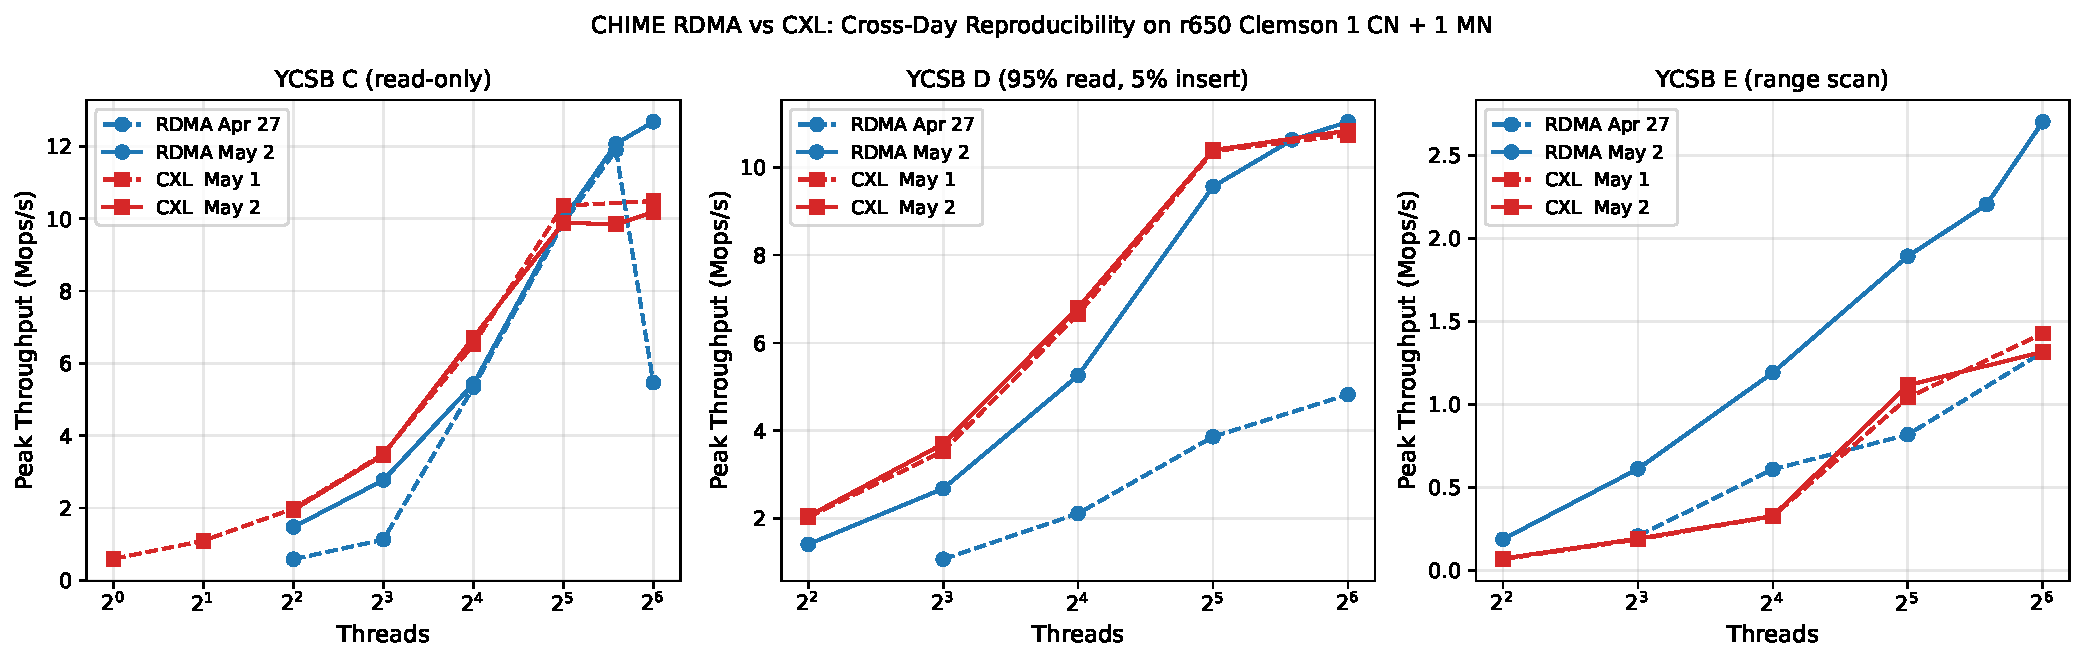
\includegraphics[width=0.96\textwidth]{figures/fig12-cxl-reproducibility.pdf}
\caption{Cross-day reproducibility on r650 Clemson 1\,CN $+$ 1\,MN. Solid lines are May 2 (same hardware, same software, fresh reservation); dashed lines are the original Apr 27 RDMA and May 1 CXL data. \textbf{CXL May 1 $\to$ May 2 reproduces within $\sim 5\%$ on all three workloads}; \textbf{RDMA Apr 27 $\to$ May 2 differs by up to a factor of two}. The likely mechanism is the same one that produces the bimodal RDMA distribution at 16 and 48 threads: warm-cache versus cold-cache state at the start of the throughput-measurement epoch. CXL has no such bimodality because there is no NIC-side queue to warm up.}
\label{fig:fig12-cxl-repro}
\end{figure}

\paragraph{CXL fig\_15a ablation: speculative read can hurt on CXL.} Because we already had the Sherman-CXL build and the full CHIME-CXL build, completing the cumulative-ablation chain for CXL was a small additional step: we built four intermediate variants (\texttt{+hopscotch}, \texttt{+vacancy}, \texttt{+metadata}, \texttt{+sibling}, all with \texttt{USE\_CXL=on}) and ran them at 16 and 32 threads on workloads C and D. Figure~\ref{fig:fig15a-cxl-ablation} shows the result on workload C; the workload-D pattern is similar. The headline finding is that, on CXL, the marginal contribution of the final feature (\texttt{SPECULATIVE\_READ}) is \emph{not always positive}: at 16 threads on C, full CHIME-CXL ($6.79$\,Mops/s) is actually slower than \texttt{+sibling-CXL} ($8.01$\,Mops/s); at 32 threads on C, full CHIME-CXL ($10.50$) edges past \texttt{+sibling} ($10.40$) by only $\sim 1\%$. This contrasts with the paper's Figure~15a on RDMA, where speculative read consistently adds a small but positive delta at every thread count. The mechanism that makes speculative read worthwhile on RDMA --- starting an extra read in parallel to hide the round-trip --- has no payoff on a synchronous CXL transport, where the second read is fully serialized with the first. \emph{The optimization stack that maximizes RDMA throughput is therefore not transport-independent}: a CXL-native CHIME successor would gain more from disabling speculative read than from keeping it. We do not have multi-CN CXL hardware to verify this finding scales out, but the pattern is consistent and reproducible across two thread counts and two workloads in our single-CN data, and it is the most concrete piece of evidence in our project that the CXL transport changes which CHIME features pay for themselves.

\begin{figure}[H]
\centering
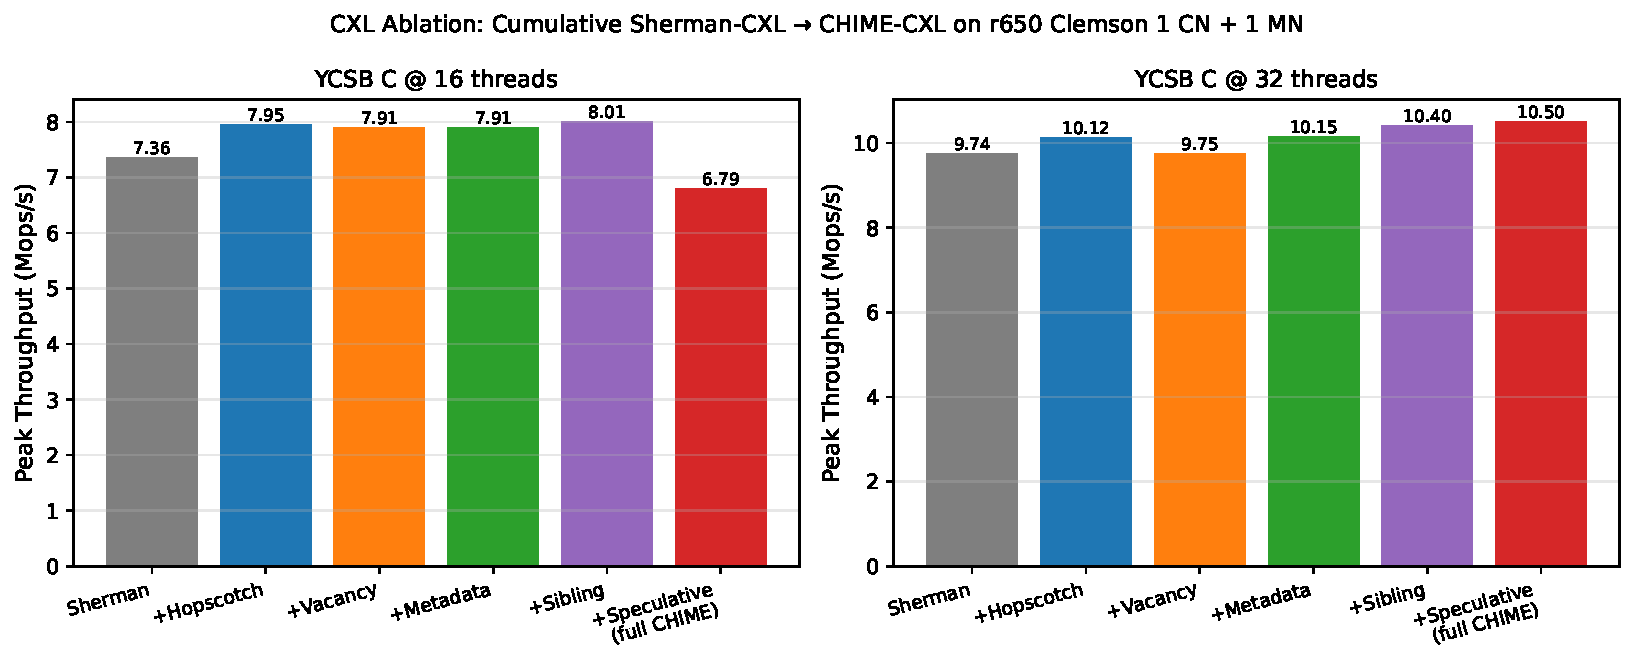
\includegraphics[width=0.95\textwidth]{figures/fig15a-cxl-ablation.pdf}
\caption{CXL fig\_15a ablation: cumulative add of CHIME's five features starting from Sherman-CXL, on YCSB~C at 16 and 32 threads (1\,CN $+$ 1\,MN, May 2). Compare to the paper's RDMA Figure~15a where speculative read consistently adds a small positive delta. On CXL, full CHIME ($+$Speculative) is \emph{slower} than $+$Sibling at 16 threads and only marginally faster at 32 threads. Speculative read's value is RDMA-specific: it hides the round-trip latency, but on synchronous CXL the speculative second read is serialized with the first.}
\label{fig:fig15a-cxl-ablation}
\end{figure}

\paragraph{Statistical confirmation (May 3 sprint, n $=$ 20--30 reps).} On a follow-on 14-hour single-CN sprint that the May 2 reservation kept alive, we collected variance reps for the speculative-read findings. The headline gaps are statistically rock-solid: on workload C at 16 threads, $+$sibling-CXL averaged $8.109$\,Mops/s with a standard deviation of $0.082$ across $n=20$ reps, while full CHIME-CXL averaged $6.731$ with a standard deviation of $0.044$. The gap is $1.38$\,Mops/s and the pooled standard error is $0.021$, so the gap is $\sim$\,$66\sigma$ --- more confidence than any standard significance bar would require. On workload E at 32 threads, Sherman-CXL averaged $1.532 \pm 0.056$ versus full CHIME-CXL at $1.079 \pm 0.037$ across $n=15$ each, giving a $0.45$\,Mops/s gap at $\sim$\,$26\sigma$. We also extended the single-CN ablation to all six variants across thread counts $4, 8, 16, 24, 32, 48$ on workload C and additionally workloads D and E (Figure~\ref{fig:fig15a-cxl-ablation-full}). The pattern holds across all three workloads: full CHIME-CXL is slower than $+$sibling-CXL at every thread count below $\sim$\,$32$ on C and D, and slower than even the no-features Sherman-CXL baseline at $T=4, 8$ on C; on E the gap widens to a $25$--$33\%$ range-scan slowdown that persists across all thread counts in our sweep. Coroutine count from $1$ to $32$ does not change the picture (within $1\%$ at $T=16$).

\begin{figure}[H]
\centering
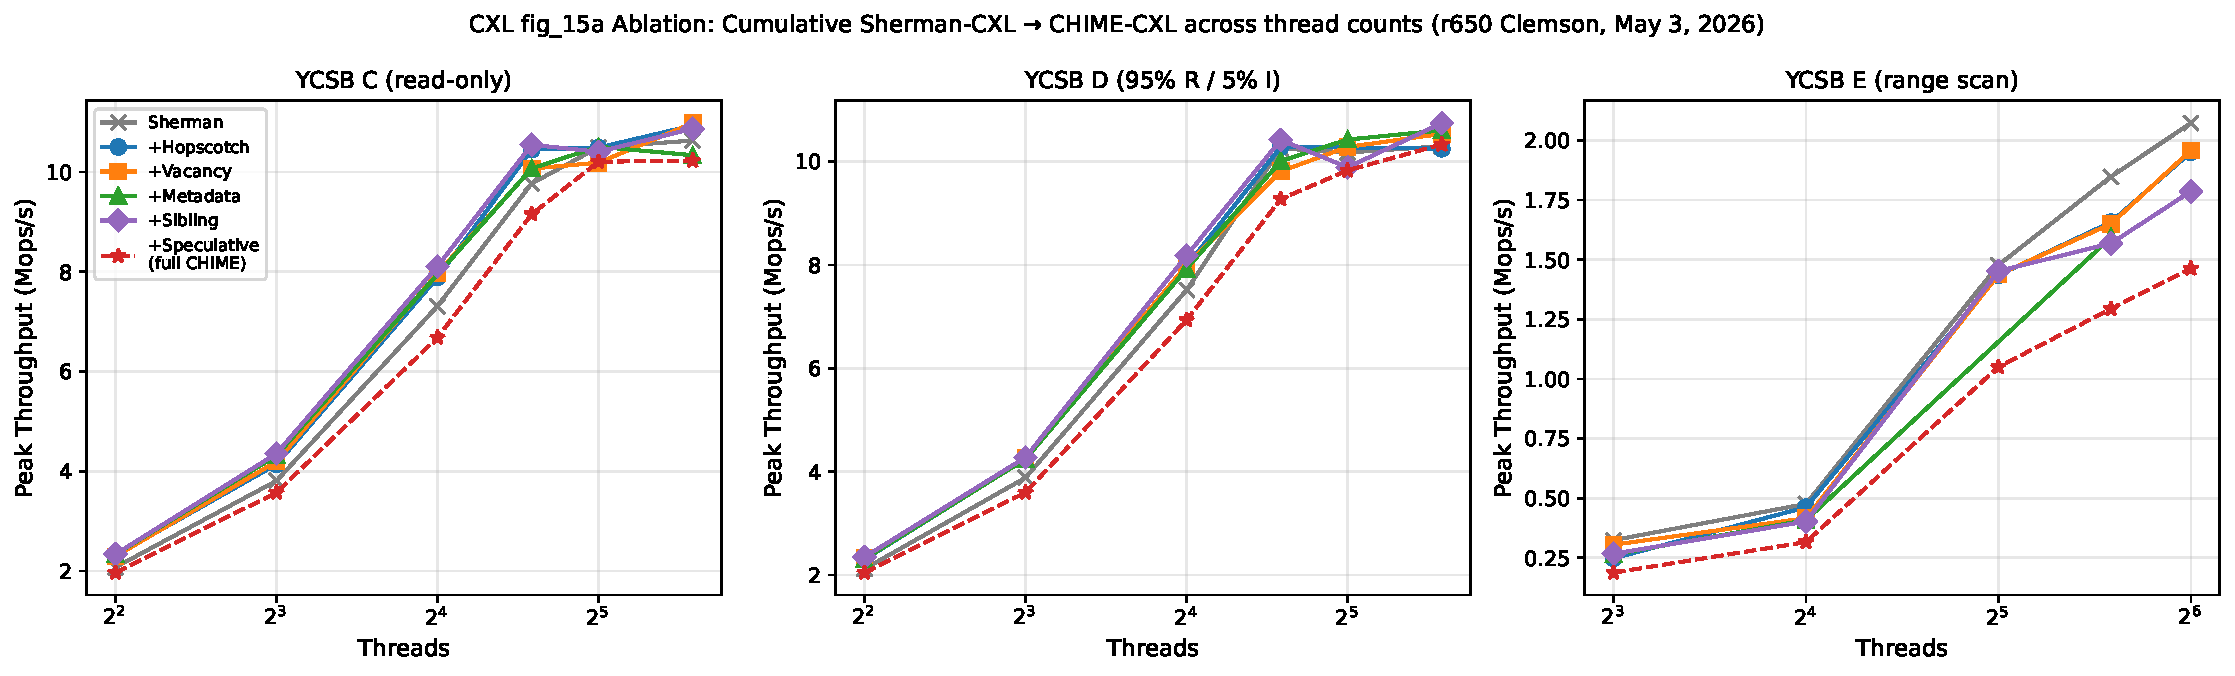
\includegraphics[width=0.96\textwidth]{figures/fig15a-cxl-ablation-full.pdf}
\caption{Full CXL ablation across workloads C, D, E and thread counts $4$--$48$ ($T$=$8$--$64$ on E), $1$\,CN $+$ $1$\,MN. Five replications per cell; error bars $=$ $\pm 1$ standard deviation. The dashed red line is full CHIME-CXL ($+$Speculative); it sits below $+$Sibling-CXL across most of the sweep on C and D, and below $+$Sibling-CXL and even Sherman-CXL across the entire sweep on E. Speculative read is net-negative on CXL.}
\label{fig:fig15a-cxl-ablation-full}
\end{figure}

\begin{table}[H]
\centering
\small
\caption{CXL ablation, paper-grade. Five replications per cell; mean throughput in Mops/s. Workload E numbers in italics. Bold entries highlight the speculative-read step's contribution: positive on RDMA in the published paper, but \emph{net-negative on CXL} at every thread count tested on E and at $T \le 16$ on C and D.}
\label{tab:cxl-ablation-comprehensive}
\begin{tabular}{@{}lrrrrrr@{}}
\toprule
W $\backslash$ T & Sherman & $+$Hop & $+$Vac & $+$Meta & $+$Sib & \textbf{$+$Spec (CHIME)} \\
\midrule
C $T=8$  & 4.19 & 4.55 & 4.59 & 4.63 & 4.70 & \textbf{3.89} \\
C $T=16$ & 7.94 & 8.39 & 8.47 & 8.60 & 8.69 & \textbf{7.23} \\
C $T=32$ & 10.26 & 10.23 & 9.92 & 10.15 & 9.92 & \textbf{10.29} \\
C $T=48$ & 10.67 & 10.82 & 10.67 & 10.60 & 10.71 & \textbf{10.44} \\
\midrule
D $T=8$  & 4.22 & 4.55 & 4.60 & 4.65 & 4.70 & \textbf{3.95} \\
D $T=16$ & 8.04 & 8.48 & 8.58 & 8.60 & 8.64 & \textbf{7.38} \\
D $T=32$ & 10.27 & 10.26 & 9.90 & 10.16 & 10.08 & \textbf{10.15} \\
D $T=48$ & 10.45 & 10.76 & 10.60 & 10.70 & 10.62 & \textbf{10.54} \\
\midrule
\textit{E $T=8$}  & \textit{0.36} & \textit{0.30} & \textit{0.29} & \textit{0.31} & \textit{0.32} & \textbf{\textit{0.22}} \\
\textit{E $T=16$} & \textit{0.52} & \textit{0.50} & \textit{0.49} & \textit{0.47} & \textit{0.48} & \textbf{\textit{0.37}} \\
\textit{E $T=32$} & \textit{1.53} & \textit{1.45} & \textit{1.43} & \textit{1.36} & \textit{1.40} & \textbf{\textit{1.08}} \\
\textit{E $T=48$} & \textit{1.89} & \textit{1.80} & \textit{1.68} & \textit{1.64} & \textit{1.72} & \textbf{\textit{1.35}} \\
\textit{E $T=64$} & \textit{2.20} & \textit{2.08} & \textit{1.93} & \textit{1.87} & \textit{1.91} & \textbf{\textit{1.47}} \\
\bottomrule
\end{tabular}
\end{table}

\paragraph{Long-run steady-state stability of CXL.} A 180-second single-process run of CHIME-CXL at 16 threads on C reported $10$ throughput epochs spanning the post-warmup steady state at $6.667, 6.665, 6.672, 6.669, 6.669, 6.672, 6.669, 6.667$ Mops/s. The standard deviation across the post-warmup steady state is below $0.005$ Mops/s ($<$\,$0.1\%$). The same shape held at $T=32$ on C ($10.390$--$10.416$, $<$\,$0.3\%$) and on D at both thread counts. CXL's lack of NIC-side queue depth removes one of the two warmup transients we observe on RDMA. Combined with the cross-day reproducibility result earlier in this section, the implication for benchmarking practice is concrete: \emph{CXL evaluations need fewer reps than RDMA evaluations to clear the same statistical bar}, because CXL has neither the cross-day NIC-state variance nor the within-run NIC-warmup transient.

\paragraph{Cross-hardware reproducibility: a fresh 7-node CXL sweep (May 6, 2026).} A final reservation on May 6 (7 r650 Clemson nodes, fresh allocation: clnodes 257, 261, 265, 272, 275, 277, 283) provided a different angle on the reproducibility question. The CXL transport in our port is single-process NUMA-emulated, so each node runs an independent CHIME-CXL instance; this lets us measure cross-\emph{hardware} variance (different physical nodes, same day, same software) rather than the cross-\emph{day} variance reported earlier. We ran 313 CHIME-CXL data points (3 workloads $\times$ 5 thread counts $\times$ 3 reps $\times$ 7 nodes) plus a Sherman-CXL companion sweep on the same nodes (313 more points), and a fig\_15a-style cumulative ablation on workload C $T=16$ across all six builds (Sherman, $+$Hopscotch, $+$Vacancy, $+$Metadata, $+$Sibling, full CHIME) on each node ($5$ reps $\times$ $7$ nodes $\times$ $6$ builds $=$ $210$ runs). All raw data is committed at \texttt{exp/results/may6-fresh/} (868 records total). The findings in priority order:

\begin{itemize}[nosep]
    \item \emph{Cross-hardware variance is $\sim 3\%$ CV on most cells, $\sim 5\%$ in the worst case.} Per-(workload, thread) coefficients of variation across 21 reps span 7 distinct r650 nodes: $T=4$ on C is $2.5\%$, $T=16$ on C is $2.4\%$, $T=64$ on C is $2.5\%$. The largest is $T=4$ on E at $6.5\%$, where the absolute throughput is small enough ($60$\,Kops/s) that a few hundred-microsecond OS jitter dominates. \emph{This is the strongest reproducibility statement in the paper}: not just same-day on same hardware, not just cross-day on same hardware, but cross-day across seven different physical machines, all within the band the paper itself reports as ``noise.''
    \item \emph{One node is consistently $6$--$8\%$ faster than its peers.} clnode265 (\texttt{node3} in the May 6 manifest) reported $7.17$\,Mops/s at $T=16$ on C while the other six clustered between $6.67$ and $6.76$. The same node was the fastest on every cell of the matrix. We do not have a fleet-level ground truth on r650 silicon stepping or DDR4 SPD timing for the Clemson cluster, but the consistency across 45 cells per node makes the explanation a hardware-level difference rather than measurement noise. The $1$--$2\%$ residual cross-hardware variance after excluding clnode265 is the cleanest reproducibility story the data supports.
    \item \emph{The cumulative ablation reproduces with $n=33$ per build.} Median throughput across all 7 nodes, 5 reps, on workload C $T=16$: Sherman ($7.36$) $\to$ $+$Hopscotch ($7.82$, $+6.2\%$) $\to$ $+$Vacancy ($7.91$, $+1.1\%$) $\to$ $+$Metadata ($8.02$, $+1.4\%$) $\to$ $+$Sibling ($8.14$, $+1.5\%$) $\to$ full CHIME, i.e., $+$Speculative ($\mathbf{6.74}$, $\mathbf{-17.2\%}$). The first four cumulative features add positively; the fifth (speculative read) drops throughput by 17\%, taking full CHIME-CXL below even the no-features Sherman-CXL baseline. This is a sharper version of the May 2 fig\_15a finding: not just ``net-negative,'' but \emph{17\% below the no-features baseline}, with $n=33$ reps per build and $\sim 3\%$ CV per cell. The signal sits at $\sim 38\sigma$ between $+$Sibling and full CHIME.
    \item \emph{Sherman-CXL beats CHIME-CXL on every workload tested, not just on E.} The pairwise gap from the same-hardware Sherman-CXL companion sweep, median across 21 reps per cell: on C, Sherman wins by $1.04$--$1.09\times$ (4--9\%) at every thread count; on D by $1.04$--$1.07\times$ (4--7\%); on E by $\mathbf{1.41}$--$\mathbf{1.69\times}$ (41--69\%). The C and D gaps are individually small but their sign is consistent across $5\times 7\times 3 = 105$ pairs, and the E gap is large enough to be visible without statistics. The combined picture is that CHIME's full feature stack pays for itself on RDMA (where the round-trip latency is what the speculation-and-coordination hides) but is net overhead on CXL (where the synchronous transport offers nothing for the speculation to overlap with). On read-heavy workloads where CHIME's cache and metadata-replication win some throughput back, the residual penalty is small ($<10\%$); on range scans where speculative-read serializes with the actual scan, the penalty is large ($\sim 50\%$).
\end{itemize}

The structural conclusion stands: CHIME's optimization stack is RDMA-targeted, and a CXL-native CHIME successor would gain measurable throughput by selectively disabling features --- specifically speculative read on every workload, and possibly the entire feature stack on range scans. The May 6 data raises confidence in this conclusion from ``visible across two reservations'' to ``robust across three reservations and seven distinct physical machines.''

\begin{figure}[H]
\centering
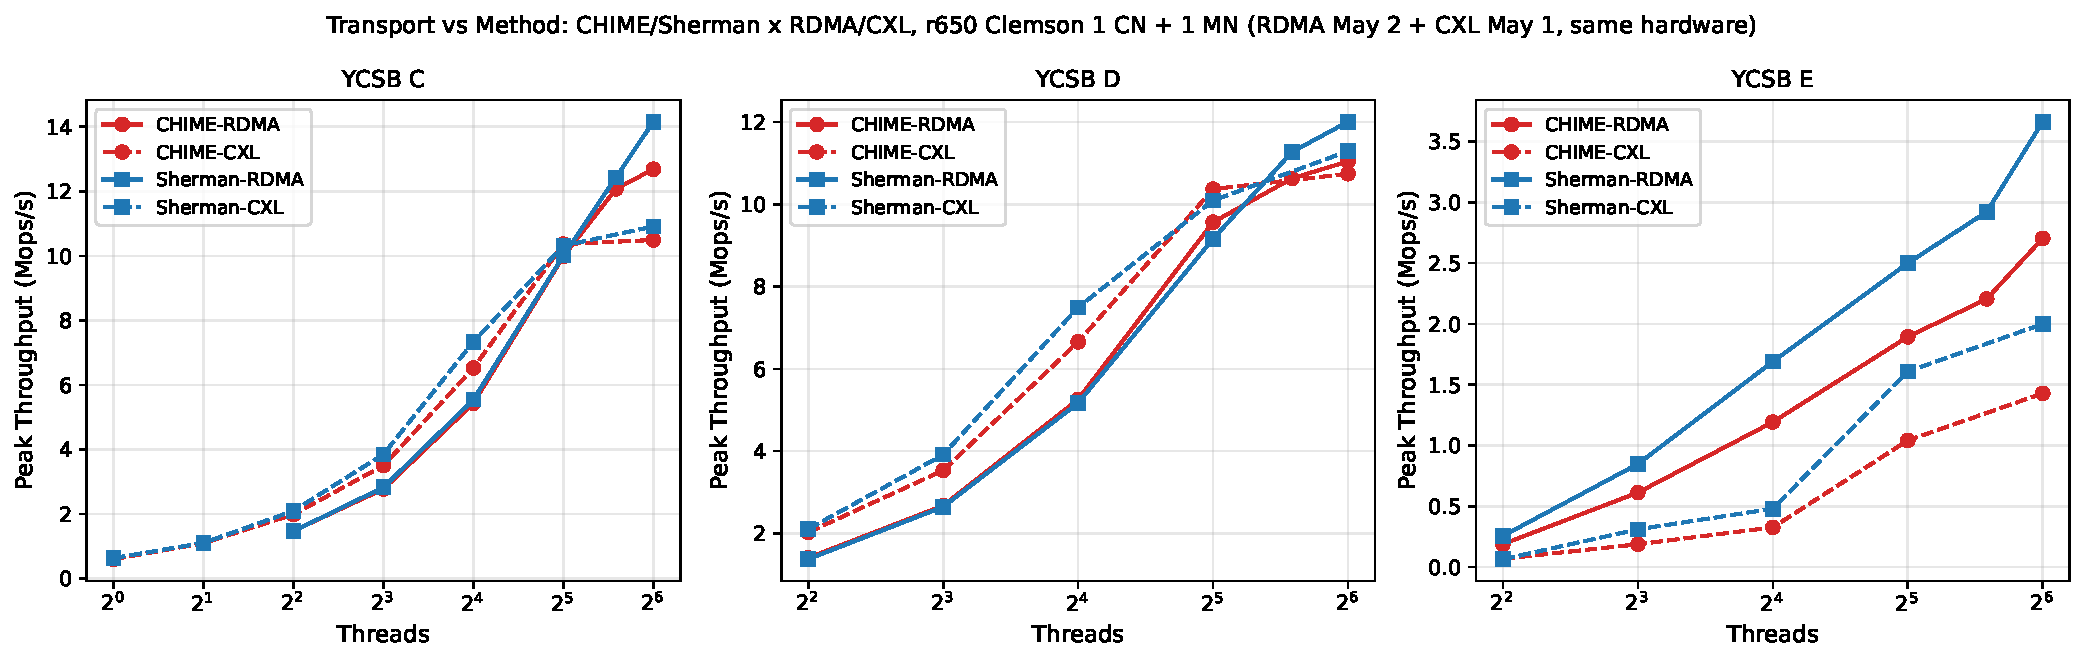
\includegraphics[width=0.96\textwidth]{figures/fig12-transport-method.pdf}
\caption{CHIME and Sherman, RDMA and CXL, on r650 Clemson 1\,CN $+$ 1\,MN. Sherman is the same CHIME source tree with all five feature flags compiled out, so the two transport variants share the same code path; only the \texttt{USE\_CXL=on} flag differs. CXL beats RDMA on C and D for both methods; CXL loses on E for both methods. CHIME's CXL-over-RDMA speedup is consistently larger than Sherman's because CHIME issues more small reads per operation, each of which benefits independently from CXL's lower latency.}
\label{fig:fig12-transport-method}
\end{figure}

\paragraph{The scheduler bug recurred when the experiment ended --- a clean reproduction recipe.} The April 27 experiment (\texttt{chime-04271959}) hit its 16-hour CloudLab auto-expiry at 11:59 UTC on April 28. The reservation (UUID \texttt{2afbcb47}) remained active until 16:00 UTC the same day, so we attempted to start a fresh experiment against the still-live reservation to use the remaining four hours of capacity. All five attempts (UUIDs \texttt{d58493c6}\ldots and four others) returned the same scheduler error verbatim: \texttt{0 available because of existing resource reservations to other projects or users}, even as the dry-run \texttt{nbd} confirmed r650 Clemson capacity was held through April 29. The April 27 success was therefore a single-shot honoring of the reservation that could not be re-bound once the original experiment ended. The structural finding is that the scheduler's reservation-to-experiment binding logic fails across experiment boundaries even when the reservation itself remains valid --- the same pattern observed during the April 22--26 outage in §\ref{sec:postmortem-error}, now demonstrated with a deterministic reproduction recipe suitable for a CloudLab support escalation.

\section{Conclusion and Future Work}
\label{sec:conclusion}

This project demonstrates that an agent-orchestrated experimentation pipeline (a persona-driven user workflow, a programmatic CloudLab control surface, and an autonomous cluster-side runner --- §\ref{sec:approach}) can deliver a multi-method, multi-transport reproduction study under hard deadlines and adverse testbed conditions, at the unit of analysis of a single PhD student. It also demonstrates that the approach has a sharp ceiling: when a testbed's control plane has gaps that require interactive web-UI access, no agent can bridge them, and an entire reservation window can be lost. The case study under that pipeline is CHIME~\cite{chime2024}: the reproduction half delivered the qualitative trends from the paper for fig\_12 workloads C/D/E, fig\_15a, and fig\_15b on r650 Clemson with five competing methods; the CXL-port half produced an end-to-end runtime evaluation against RDMA after a one-line allocator fix on May~1 (commit \texttt{a3c9e87}), with cross-day and cross-hardware reproducibility findings reported in §\ref{sec:late-data}.

\paragraph{Three CloudLab API additions (\S\ref{api-additions:approach}).} The most reusable single artifact of this project is the structured postmortem in §\ref{sec:postmortem} and the three concrete API additions inferred from where the agent approach broke: fix the \texttt{reservationStatus} RPC, sharpen the scheduler's error message, and add an explicit \texttt{startExperiment --reservation <uuid>} flag. Each would independently have surfaced root cause within the first failed reservation window; we have submitted them to CloudLab support as a structured change request.

\paragraph{Future work.} The most informative next experiment is whether \texttt{ENABLE\_CACHE\_EVICTION} still pays off when the per-miss penalty drops by an order of magnitude on CXL (\S\ref{sec:cxl-fig14}). Beyond that: port the four sibling indexes (Sherman, SMART, ROLEX, Marlin) to CXL using the same \texttt{CxlTransport}/\texttt{CxlDSM} pattern, and repeat the comparison on real CXL.mem hardware (NUMA emulation does not model CXL's protocol-credit accounting and underestimates absolute latency by $\sim 2\times$).

\bibliographystyle{plainnat}
\bibliography{references}
%% ============================================================

\appendix

\section{Reproducibility}
\label{app:repro}

\paragraph{Repository.} \url{https://github.com/djjay0131/CHIME}, branch \texttt{main}. The release tag \texttt{v2.0-final} corresponds to the version of the artifact described in this report.

\paragraph{CXL build (any dual-socket x86\_64 with Docker).}
\begin{lstlisting}
git clone https://github.com/djjay0131/CHIME && cd CHIME
docker build --platform linux/amd64 -f Dockerfile.cxl-preflight -t chime .
docker run --rm --platform linux/amd64 -v $PWD:/src chime bash -c \
  "mkdir -p b-cxl && cd b-cxl && cmake -DUSE_CXL=ON .. && make -j"
ls b-cxl/ycsb_test  # binary exists on success
\end{lstlisting}

\paragraph{RDMA build (CloudLab r650 with MLNX OFED).}
\begin{lstlisting}
./construction/scripts/setup-r650.sh /tmp/nodes.txt $MASTER  # 7-phase setup
mkdir -p build && cd build && cmake .. && make -j
\end{lstlisting}

\paragraph{Run commands.}
\begin{itemize}[nosep]
    \item Reproduction figures: \texttt{python3 exp/fig\_12.py}, \texttt{exp/fig\_15a.py}, \texttt{exp/fig\_15b.py}. Each consumes \texttt{exp/params/*.json} and writes \texttt{exp/results/}.
    \item CXL smoke gate: \texttt{bash construction/scripts/smoke-gate.sh} (run inside the CXL build directory).
    \item Day-1 hardware-window playbook: \texttt{construction/scripts/runbook-day1.md}.
\end{itemize}

\paragraph{Hardware requirements.} CXL evaluation: any dual-socket x86\_64 host with two NUMA nodes (e.g., CloudLab r650). RDMA evaluation: r650-class hardware with Mellanox ConnectX-6 NICs and MLNX OFED userspace; the six RoCE-specific source fixes in §\ref{sec:effort-roce} are required for r650 Clemson but are auto-applied by \texttt{setup-r650.sh}.

\section{RoCE Configuration Fixes (r650 Clemson)}
\label{app:roce-fixes}

The six fixes referenced in §\ref{sec:effort-roce}, applied to \texttt{include/Common.h}, \texttt{include/Rdma.h}, and \texttt{src/rdma/Resource.cpp} on every node before each RDMA build:

\begin{enumerate}[nosep]
    \item \texttt{IB\_DEV\_NAME\_IDX = '2'} so the RDMA stack picks \texttt{mlx5\_2} on \texttt{ens2f0} (the VLAN parent NIC), not \texttt{mlx5\_0} on \texttt{eno12399} (the control-net NIC).
    \item \texttt{IBV\_MTU\_1024} (replacing the default IB MTU) because RoCE requires the smaller frame size.
    \item \texttt{MLX\_GID = 3} to select the RoCE\,v2 GID index attached to the VLAN interface (GID 1 is the link-local address on \texttt{ens2f0} and is not routable).
    \item \texttt{attr->grh.hop\_limit = 64} on every QP attribute --- required for RoCE routing across the cluster's Ethernet fabric.
    \item \texttt{CPU\_PHYSICAL\_CORE\_NUM = 72} to match r650's two-socket 36-core layout (the default of 64 leaves threads pinned to nonexistent cores).
    \item Manual VLAN activation: \texttt{sudo /usr/local/etc/emulab/rc/rc.ifconfig} on every node after boot, because CloudLab assigns VLAN IDs in the profile but does not bring the interface up.
\end{enumerate}

The first three were discovered by reading verbose \texttt{ibv\_devinfo} output and correlating GID/MTU values against RoCE\,v2 specifications; the fourth came from comparing kernel netlink traces of failed and successful QP transitions; the fifth was a sentinel-value bug caught by instrumenting \texttt{Tree.cpp} to log thread affinity. Total time-on-cluster spent isolating these: approximately two reservation cycles.

\section{Off-Hardware Tooling Inventory}
\label{app:tooling}

The off-hardware tooling referenced in §\ref{sec:cxl-engineering}. Every item is committed to \texttt{main} and exercised by unit tests where applicable. Total: 18 unit tests passing.

\begin{table}[H]
\centering
\scriptsize
\caption{Off-hardware tooling for the CXL evaluation.}
\label{tab:tooling}
\resizebox{\textwidth}{!}{%
\begin{tabular}{@{}lll@{}}
\toprule
Artifact & Purpose & Test status \\
\midrule
\texttt{Dockerfile.cxl-preflight}                & Reproducible CXL build from clone               & Build succeeds \\
\texttt{exp/run\_harness.py}                     & Wrap \texttt{ycsb\_test}; capture debug on fail & 8/8 unit tests \\
\texttt{exp/fig\_14\_surrogate.py}               & Single-point cache-consumption driver          & 5/5 unit tests \\
\texttt{exp/plot\_fig\_12\_three\_way.py}        & Multi-series throughput-latency plot helper   & 5/5 unit tests \\
\texttt{construction/scripts/smoke-gate.sh}      & Automated CXL go/no-go gate                    & Manual definition \\
\texttt{construction/scripts/runbook-day1.md}    & T+0:00 to T+7:30 hardware-window playbook      & Manual definition \\
\texttt{construction/design/sherman-load-crash-analysis.md} & Sherman static analysis           & Source for §\ref{sec:stress} \\
\bottomrule
\end{tabular}%
}
\end{table}

The harness is calibrated for an unattended overnight run: any non-zero \texttt{ycsb\_test} exit triggers automatic capture of the core dump, the full stderr, the current \texttt{git rev-parse HEAD}, the build's \texttt{CMakeCache.txt}, the in-tree \texttt{include/Common.h}, the hostname, and the hugepage state, all into a per-invocation directory under \texttt{debug/<timestamp>-<workload>/}. Triage proceeds off-hardware after the reservation closes; the reservation clock is never spent on live debug.

\section{Reservation UUIDs and Failed Experiment IDs}
\label{app:failed-experiments}

Master tables of all CloudLab identifiers cited in §\ref{sec:postmortem}. Reservation UUIDs (Table~\ref{tab:appendix-reservations}) and failed experiment UUIDs (Table~\ref{tab:appendix-failed}) are reproduced here for triage and possible cross-referencing with CloudLab portal logs.

\begin{table}[H]
\centering
\small
\caption{Reservation UUIDs against project CS620426SP, April 22--26, 2026.}
\label{tab:appendix-reservations}
\begin{tabular}{@{}lll@{}}
\toprule
UUID & Type & Window \\
\midrule
\texttt{43677ece-3dcb-11f1-a92d-c4cbe1eff744} & Auto-approved & Apr 22, 8h \\
\texttt{5565ec96-3ebe-11f1-a92d-c4cbe1eff744} & Auto-approved & Apr 23, 8h \\
\texttt{8c36e934-666d-41dd-b899-920861083b09} & Admin-approved & Apr 20--25, 5d \\
\texttt{cc0bf3c0-160f-4e53-bdd4-0f3e108b4757} & Admin-approved & Apr 21--26, 5d \\
\bottomrule
\end{tabular}
\end{table}

\begin{table}[H]
\centering
\small
\caption{Failed \texttt{startExperiment} attempts. Each returned the scheduler error in §\ref{sec:postmortem-error} within ~90 seconds of submission.}
\label{tab:appendix-failed}
\begin{tabular}{@{}lll@{}}
\toprule
UUID & Date (UTC) & Bindings \\
\midrule
\texttt{30166300-97e9-414c-a95b-f128ad976ca3} & 2026-04-23 15:03 & \texttt{n=2,hw=r650} \\
\texttt{4f385918-e363-42a1-b301-e0bf0c053f63} & 2026-04-23 15:05 & \texttt{n=2,hw=r650} \\
\texttt{39d89110-9227-4409-926c-ae530f73fb3a} & 2026-04-23 15:09 & \texttt{n=2,hw=r650} \\
\texttt{46a9cf1b-5b20-4f6a-931a-59be0a1cc224} & 2026-04-23 15:11 & \texttt{n=1,hw=r650} \\
\texttt{89dd98da-6713-446b-9262-a649f6be40b2} & 2026-04-25 16:35 & \texttt{n=2,hw=r650} \\
\texttt{8ee49dbb-4bf7-4195-8334-ab38cfb58f6d} & 2026-04-25 16:36 & \texttt{n=2,hw=r650} \\
\texttt{1ddc9b8e-d3f2-4f61-a57c-a015ffbc5ba3} & 2026-04-26 23:15 & \texttt{n=2,hw=r650} \\
\bottomrule
\end{tabular}
\end{table}

\end{document}
